%
% Niniejszy plik stanowi przykład formatowania pracy magisterskiej na
% Wydziale MIM UW.  Szkielet użytych poleceń można wykorzystywać do
% woli, np. formatujac wlasna prace.
%
% Zawartosc merytoryczna stanowi oryginalnosiagniecie
% naukowosciowe Marcina Wolinskiego.  Wszelkie prawa zastrzeżone.
%
% Copyright (c) 2001 by Marcin Woliński <M.Wolinski@gust.org.pl>
% Poprawki spowodowane zmianami przepisów - Marcin Szczuka, 1.10.2004
% Poprawki spowodowane zmianami przepisow i ujednolicenie 
% - Seweryn Karłowicz, 05.05.2006
% Dodanie wielu autorów i tłumaczenia na angielski - Kuba Pochrybniak, 29.11.2016

\documentclass[en]{pracamgr}

\autor{Mateusz Bajorek}{385122}

\title{Analysis and visualization of programmers’ activities during their workday}
\titlepl{Analiza i wizualizacja aktywności programistów w ramach ich dnia pracy}

\kierunek{Computer Science}

% Praca wykonana pod kierunkiem:
% (podać tytuł/stopień imię i nazwisko opiekuna
% Instytut
% ew. Wydział ew. Uczelnia (jeżeli nie MIM UW))
\opiekun{dr Robert Dąbrowski\\
  Institute of Informatics\\
  }

% miesiąc i~rok:
\date{December 2022}

%Podać dziedzinę wg klasyfikacji Socrates-Erasmus:
\dziedzina{11.3 Informatics, Computer Science}

%Klasyfikacja tematyczna wedlug AMS (matematyka) lub ACM (informatyka)
\klasyfikacja{D. Software}

% Słowa kluczowe:
\keywords{programming process analysis, programming process visualization, keystroke dynamics}

% Used Latex packages
\usepackage{xurl}
\usepackage{hyperref}
\usepackage[all]{hypcap}
\usepackage{xcolor}
\usepackage{graphicx}

% Tu jest dobre miejsce na Twoje własne makra i~środowiska:
\newtheorem{definition}{Definition}[section]

% koniec definicji

\begin{document}
\maketitle

\begin{abstract}
Similarly to another professions, programmers create their own working style. It can be characterized by
different phases of the day, splitting tasks into a few chunks, taking breaks, or focusing on a few
projects at the same time. In this thesis, I analyze if there exist links between programmers preferences
and the spectre of their duties for example, if it is true that front-end programmers work usually in the
evenings. For this purpose, I conduct a research scheme on a sample of programmers with the help of a self-created software tool for gathering anonymized data (including the number of projects, time of
activities, programming languages or particular frameworks usage). The end result of this thesis, are the
conclusions from the analysis of the aforementioned data with included visualizations. The tool used
in the thesis is shared publicly for the willing actors to independently verify my end results by
re-running the experiments or running new ones to gather new information for example about potential
improvements in programmers efficiency.
\end{abstract}

\chapter*{Acknowledgements}
\textcolor{red}{TODO}

First of all, I would like to thank my supervisor PhD Robert Dąbrowski for expert guidance during the "Software Optimization, Visualization and Analysis" (SOVA) seminars. His help in the university administrative procedures involving this thesis and overall assistance and patience in overcoming various obstacles was invaluable. 
% patience, many tips, critical insight

Another lecturer present during the seminars was Prof. Krzysztof Stencel who provided me with essential advice which I appreciate greatly. I also thank for his attempts at help in gathering the data for me.

Apart from the leaders of the seminars, I must mention my colleagues who were present at my presentations. This was the time when we shared our remarks on each other's work. My thesis would not be the same without their input during these discussions.

I especially thank (highlight from my colleagues) Małgorzata E. Z. Galińska (née Biegała) for testing and assistance with debugging of my addon.
% for being the first to test

My former employers and dear friends M. Asberg (CEO NewNative) and R. Dembkowski (CEO RadCode) for the help with gathering the data.
% and every employee who decided to share the data
% using their professional contacts and oportunities

I thank everyone who decided to share their data with me to proceed with my research project.

I am grateful for the Faculty of Mathematics, Mechanics and Informatics of the University of Warsaw for being able to study Computer Science and conduct my research there.

Lastly, my thanks go to my friends and family for their immense patience and unwavering support (also financial and emotional).

\begin{flushright}
Warsaw, December 2022

Mateusz Bajorek
\end{flushright}


\tableofcontents

\chapter{Introduction}

Programmers job focuses on developing computer software through all phases including design, testing and maintenance. These processes are executed according to the principles of performance, reliability and security \cite{Sto21ProgrammersDo}. With the industry maturing, upholding these rules in ever-expanding projects have become crucial to fulfill growing needs stated i.a. in software level agreements (SLAs). One of the answers to that have been the agile software development \cite{Gro21SDMHistory}, where actions like joining regularly scheduled team meetings, contacting clients or attending conferences have been universalized. Nevertheless, writing code has remained a key part of programmers job for the majority of them. In my study, I focus on analyzing and visualizing the exact process of writing software in an integrated development environment (IDE), largely omitting the other aforementioned aspects of being a programmer.

Research in the relevant areas differs depending on the context that is industrial or educational. Tracking of programmers time happens to be an essential part of the job in the IT industry. The reports provided by programmers are the basis for calculating a salary or even deciding the future of an employee by the management. For many programmers it may be hard to determine which activities constituted billing time or if different activities should be treated differently. In my own experience, hard to fix bugs or complicated issues solving which took many trials and errors happened to be particularly hard when it comes to calculating the exact amount of billing hours it took me and how to prove this reported effort to my employer. Those obstacles constituted my initial desire to explore the domain of programming process analysis and visualization. Nowadays there exist tools that measure the time automatically and compile the reports with almost no additional human effort.

In the industry there is less focus on the detailed analysis of the process of writing the code and more on the activities done during the whole workday. Process of writing the code is more of a concern for educational research and IDE development companies like JetBrains who want to know how users interact with their products and how to make them more ergonomic. In educational research people try to evaluate students based on their typing behavior. Apart from that, it's possible to authenticate users based on their typing characteristics.

% It was then I came up with researching this area a bit further. My idea was to track programmers activities even before they create any meaningful output. Of course, you could argue that the paradigms of continuous integration already solve this problem, however at the heart of my concerns lied the relatively high granularity of the data, which would be practically unachievable just by utilizing common paradigms (you do not imagine a programmer committing her/his work to git every minute or even more frequently without a high nosedive of her/his productivity).

The thesis contains 5 chapters and appendices. In the chapter \ref{r:background} there are studied basic concepts and related works both in analysis and in visualization techniques. The chapter \ref{ch:methodology} describes the tool used to gather and analyse the data. In the chapter \ref{ch:results} the results are presented and in the next one \ref{ch:discussion} they are discussed. The last two chapters conclude the whole thesis with suggestions for future work \ref{ch:conclusions} and provide links to the additional published materials \ref{ch:publishing}. I clarify that the pronoun “I” used in this thesis refers to its author.

% Say what it is about and what not. Say what data you use and which not. Say what to expect.

% Say that by activities you mostly mean just keystrokes.

% It's important to mention here that I am not interested in resources of data such as surveys, and only the factual data sources as there exists evidence that the programmers perception is inconsistent with the real data. Reference here.

% Mention that educational approaches can be used in the industry in the future.

\chapter{Background}\label{r:background}

\section{Basic concepts with their applications}

Throughout the thesis I use terms distinctive to biology, software engineering or IT industry. I have decided to highlight some of them due to their importance and ubiquity in my thesis or in the related works. Apart from the essential definitions, I provide the applications together with my motives to utilize this terminology.

\begin{definition}\label{def:circadian_rhythm}
\emph{Circadian rhythms} are a set of physiological changes that follow a cycle of roughly 24 hours. These processes are governed by a biochemical clock in the brain that receives the fluctuating light during the day and at night. They fundamentally influence person's activity levels at different hours. \cite{Rep02CircadianTiming}
\end{definition}

Circadian rhythms enable humans to follow day cycles. It is an important concept in my thesis since I mainly consider programmers work on the basis of separate days. Within a single day, there are expected differences of behavior between programmers, partially explainable by a notion of chronotypes.

\begin{definition}
\emph{Chronotype} is a natural tendency of a person toward increased or decreased activity at certain parts of the day. It is closely coupled with human's circadian rhythms. \cite{Roe03Chronotypes}
\end{definition}

The theory of individual's chronotype is a major reason why some developers exhibit greater activity during earlier parts of the day while the others during the later ones. Such a phenomenon occurs obviously within the confines of social norms. Programmers of late chronotypes (the so-called "night owls") are subject to the same common working hours as the ones of early chronotypes (the so-called "morning larks"). Thus, the true extent of individual's chronotype can be further studied by analyzing weekend activity or volunteer work on open-source projects (which may, in fact, still be influenced by external factors). Nevertheless, chronotypes remain a vital factor in determining programmers productivity peaks and slumps which are in the focus of my thesis.
% \textcolor{red}{TODO! REF}

\begin{definition}
\emph{Time tracking} refers to a company policy regarding logging time of its employees. The reports compiled in this process present a summary of time spent on each given task by an employee. \cite{Fed21TimeTracking}
\end{definition}

In ordinary company operations chronotypes are not a matter of general concern. What undoubtedly matters is the eventual completion of tasks assigned to each programmer. In order to secure this goal, the systems of time tracking are introduced to software development teams. This way superiors can estimate time required to achieve milestones and compensate employees fairly according to their performance. Several techniques of time tracking are comparable to the ones used to investigate chronotypes. My belief is that integrating the idea of a chronotype into time tracking programs may contribute to improved deadline estimates and more accurate assessment of programmers conduct.

\begin{definition}
\emph{Keystroke dynamics} is a research area concerning the rhythm of typing. It generally involves recording person's keystrokes with their timestamps in order for the gathered data to be further analyzed. \cite{Lei19Dissertation}
\end{definition}

The domain of keystroke dynamics is imperative for examining human behaviour at a computer keyboard. Since capturing and inspecting keystrokes are my main research methods, findings pertinent to keystroke dynamics provide an indispensable help in my thesis.

\begin{definition}\label{def:programming_process}
\emph{Programming process} relates to the way how a particular programmer develops a given piece of software. This process can be observed by tracking the programmer's actions linked to typing the source code on a keyboard. \cite{Mat13PPV}
\end{definition}

% \textcolor{red}{TODO! weird!}
Tracing programming process through the means of keystrokes capturing is my main objective. It is potentially a great observation point for chronotypes. It is also a point of concern for time tracking. Thus, it can be seen as a handy concept that clusters together multiple ideas mentioned earlier.

\begin{definition}
\emph{Granularity} of the data refers to the number of recorded data points per unit of time.
\end{definition}

In short, data granularity is simply the relative density of data points. Greater granularity (denser data) allows for potentially more extensive studies, while lesser granularity (sparser data) saves computer resources. This and other dilemmas regarding the data granularity aspect in research studies are examined in literature \cite{Vih14CodeSnapshotGranularity}.

\begin{definition}
\emph{Code snapshot} is a saved state of programmer's work at a specific point in time. It typically contains a copy of all the source code that was written until the time of capturing the snapshot. \cite{Jad06NoviceCompilationBehaviour}
\end{definition}

% \textcolor{red}{TODO! weird!}
Storing a sequence of code snapshots gives an exceptional insight into the programming process. It may be of different granularities with keystroke level comprising dense data points and git commits - sparse ones. In the literature code snapshots may also relate to the gathered metadata (like timestamps of user actions). Thus, it can be said that my system in fact gathers subsequent code snapshots.

My work is focused on analyzing chronotypes of different programmers and finding relations between chronotypes and various factors like programming languages used. The chronotypes may exhibit different characteristics like the frequency and length of breaks, or amplitude of activity peaks. Apart from the chronotypes, I am interested in the particular actions themselves, especially the difference in deletes and additions. To see if there is some kind of variation in this regard between programmers or clusters of programmers within a given language.

\section{Tracking programmers time in the IT industry}

In many areas of the IT industry, programmers salaries are the most significant expense
% todo ref
and not the computation time (electricity bills, server maintenance etc.). In such a case, effective management of these human resources becomes a crucial task for keeping finances of a company in check. That is why it is essential to know exactly how much many hours need to be spent for each programmer and on which tasks. For this purpose many tools were created to generate relevant reports for the employer's oversight on the company and for the employees themselves to motivate them to earnest effort.

The tools like Trello \cite{Trello}, Jira \cite{Jira}, YouTrack \cite{YouTrack} allow for manual time tracking. The programmers are required to manually mark their progress. They are tightly coupled with software development methodologies (established ways of navigation through each phase of the software development \cite{Con92SDM}). Handling agile frameworks such as Kanban and Scrum is especially important for these tools.

Nevertheless, there are also tools which help with automated time tracking. Such tools inlcude Timely \cite{Timely} and Tempo \cite{Tempo} products. They track user actions and evaluate them using different techniques (including those based on machine learning) to label them accordingly. This way the users can save the time on filling out the reports, especially thanks to built-in integrations with Jira etc. Another interesting solution is to integrate dashboards directly into an IDE. Notable examples of that approach include WakaTime \cite{WakaTime} and CodeTime \cite{CodeTime}. The visualizations and statistics that these tools conveniently generate for the IDE users are comparable to those available in my tool. However, one of my main premises was to ensure the availability and security of the gathered data adhering exactly to my specification. Thus, I have decided to built my own tool according to the aforementioned principles.

The agile software development methodologies mentioned above (Kanban and Scrum) utilize special dashboards with clearly described tasks for programmers. They represent an interesting way of visualizing activities of developers. My thesis does not cover detailed labeling of activities which is required by those techniques. Nevertheless, it is a concept worth noting for potential further research. The emergence of the automated time tracking tools (e.g. Timely and Tempo products) show that the IT industry is attentive to the developments in the area of sophisticated analyzing and visualizing of programmers' activities. I hope my thesis also gives some insight into this matter.

% To do I should probably mention here that I Focus here on the methods related to capturing keystrokes data or input so to say. Want somebody there are some inspiring startups we'll see in the internet will maybe Explore More tools related to time tracking.

\section{Usage of programmers data in research}

% \textcolor{red}{TODO}
Analysis of gathered programmers data is a vibrant area of research. I would like to make a quick overview of such research, especially this most relevant to my thesis.
% \textcolor{red}{TODO: mention literature review studies and in visualization as well!}

Zavgorodniaia et. al. \cite{Zav21MorningEvening} collected keystroke data from two groups of introductory programming students (European and American) using a custom IDE. This data allowed the research team to search for the activity patterns associated with distinct chronotypes. They identified four chronotypes isolated by Putilov et. al. \cite{Put19FourChronotypes} that is morning, napper, afternoon, and evening. The difference in scores was the most noticeable within the US context, where morning persons achieved the highest exam scores. Comparing the contexts, it was observed that European participants usually started their work earlier than their American counterparts. Researchers stipulated that the coincidence of their results with the prior published research does not prove that students’ circadian rhythms and diurnal preferences are the sole reason for their activity patterns. Social factors like rigid schedules or external duties might have impacted the conclusions since the surveys for such factors were not taken as part of the experiments.

Claes et. al. \cite{Cla18NightWeekend} examined programmers work patterns by analyzing version control commits from multiple software projects. The researchers found that typically developers follow the standard circadian rhythm where effort is concentrated in the morning and in the afternoon. Unsurprisingly, they observed characteristic dips in activity around the lunch time (11 or 12 o'clock depending on the project) and much bigger ones during the weekends. The myth of programmers being night owls was not confirmed since according to the data the median 8-hour working day is placed between 10 and 18 o'clock. In addition, the data showed that two thirds of developers work primarily within the office hours. The researchers found some evidence that activity outside the normal office hours is correlated with non-paid (hobby) work.

Robinson \cite{Rob17LangsUsedAtNight} examined in his article the data from Stack Overflow about visits to the site. Stack Overflow is a popular platform where developers ask and answer technical questions. The author of the article decided to inspect developers programming behavior assuming a strong link between Stack Overflow and programming activity. Not surprisingly, the peak activity was observed during the weekdays within the standard 9-to-5 time period (adjusted for local time zones). Moreover, a dip in traffic was observable at 12 p.m. coinciding with a typical lunch hour. On weekends such a dip did not exist. Across several programming languages there were noticed slight differences in hourly trends, that is some of the languages were e.g. associated with statistically earlier or later times of activity. The author also highlighted the technologies that were relatively most used within or outside the typical working hours (9-to-5). Multiple Microsoft (a major IT company) products demonstrated high percentages of usage within the working hours, while Haskell (a functional programming language), Firebase (an application development platform) and Unity (a game engine) outside of them. In addition to that, there was analyzed usage in the morning and the afternoon, and found a general correlation between usage within working hours and in the morning. At the end, it was discovered that cities known for remote work exhibit a bigger number of late chronotypes comparing to traditional software/business centers with locally employed programmers.

Silge \cite{Sil17LangsUsedOnWeekends} explored the diversity of questions that are posted on weekdays and weekends. She noticed that some languages become more popular during weekends (with regards to the relative frequency on weekdays vs on the weekend). There are also trends of diversion in these statistics throughout time which may suggest maturing of certain technologies (moving activity from weekends to weekdays) or going more mainstream with hobbyists (moving activity from weekdays to weekends).

% TODO reconsider wording
\section{Tools for gathering programmers' data}


% Timely - for billing not for keystrokes tracking
% no keystroke monitoring - mentioned as a feature (no "creepy" surveillance tactics)

% and why I'm not using them - that is those tools above

% Difference in convenience

% TODO reconsider wording and structure
\section{Tools for visualizing the programming process}

% Mention literature review
% TODO How it can be done - different means like SCSs etc.
Visualization of software is a vigorously studied area. \cite{Mat16SoftwareVisualizationReview} It concerns mainly representations of software structure, behavior and evolution \cite{DieSoftViz}. In my thesis I am mostly interested in the last point with emphasis on visualization of the programming process by analyzing keystrokes. The different takes on this matter are presented below. 
% \textcolor{red}{TODO expand}

Balzuweit et. al. \cite{Bal13SnapViz} developed a prototype tool named \textbf{SnapViz} which aims to standardize the systems for displaying snapshot data gathered from programming students. The tool consumes timestamped data points containing information about a student, a task, the student's score achieved on the task with the relevant code snapshot, and a label (e.g. an error message). Thanks to the data, a plot is generated with time and date axes, that presents how individual's solutions evolved in time. This way it can be observed how many attempts a student took and if the score increased gradually or with a spike. The authors of the article hoped to spur discussion and they actually succeeded judging by references appearing in some of the papers mentioned below.

% \textcolor{red}{TODO rewrite}
Shrestha et. al. \cite{Shr22CodeProcess} presented a tool called \textbf{CodeProcess} for visualizing the programming process \ref{def:programming_process}. The main point of the tool is to show the order in which the source code was written. The tool allows to see the keystroke data in a plot arranged from each character added. 
% \textcolor{red}{TODO expand previous}
The authors conducted a study to evaluate the usefulness of the tool for educators. They came with multiple potential areas for the tool including grading assistance, determining student's approach to the problem (top-down or bottom-up), detecting plagiarism, or finding struggling students in need of support. Apart from teachers, students could use the tool to reflect on themselves to see different approaches in overcoming potential obstacles. The authors state that the process of analyzing the plots could be enhanced by ML to enable automated reasoning (e.g. for plagiarism screening). Apart from education, the ideas behind the tool are expected to be used in the professional context for code reviews and self-growth of programmers.

Matsuzawa et. al. \cite{Mat13PPV} developed a tool named \textbf{Programming Process Visualizer} (\textbf{PPV}) based on the Personal Software Process (PSP) framework. It comprises a set of techniques to help engineers and their organizations improve their performance through a disciplined approach to measuring and analyzing their work \cite{Hum96PSS}. The PPV software allows students to analyze their programming process after completing a programming task. The tool provided students with the replay ability, so they could see the animation of writing the source code. In parallel, the metrics are calculated, including number of lines, working time and other information about compilations and runs. A notable feature crucial for the PSP is the ability to provide labels for the subtasks, that is pieces of code, for what students actually attempted to achieve by writing them. This way students are able to estimate the time they thought it would take them to complete an assignment and compare it with the real time span. The researchers tested their tool empirically on the students and it gave them promising results with the students providing positive responses.

Biehl et. al. \cite{Bie07FASTDash} created a tool called \textbf{FASTDash} to enhance team awareness in software development projects. They intended to achieve that by deploying a visualization that provides information about current activities of each programmer. This way a developer can quickly learn which team members are working on each files or even exactly on which parts of code like classes or methods. The developers can even provide comments for better understanding. One of the more obvious advantages of this solution is to mitigate the risk of conflict situations. The tool was tested in an experimental environment with promising results and some developers continuing to use it afterwards.

Lyulina et. al. \cite{Lyu21TaskTracker} developed a toolkit named \textbf{TaskTracker} for collecting and analyzing data of student programming process. The gathered data includes code snapshots of high granularity (even with 1 character change) and other user actions taken within the IDE based on the IntelliJ Platform. The tool allows for tracking solving a fixed number of predefined tasks in various programming languages. The authors created and published a dataset by tracking activities of 148 participants. It is interesting to see that the tool can be used to detect plagiarism similarly to one of the tools above.

% \textcolor{red}{TODO! More!}
Norris et. al. \cite{Nor08ClockIt} introduced a tool called \textbf{ClockIt} for monitoring student programming practices. It logs opening and closing projects or packages, compilation and run events, as well as files deletions and changes. The gathered data is presented in summary visualizations of compilation statuses and invocation outcomes within chosen time periods. The tool provides also the activity graph with the total count of events in time and the project growth graph with the total number of lines of code and comment in subsequent days.

The tools listed above differ in the granularity of the data gathered and the scope of the code base analysed. Some of them work on the keystroke level while the other analyze git commits. There are those focusing only on one source code file and those analyzing the entire code repository. Instead of attempting to utilize one of the available technologies, I have decided to build my own tool with the chosen level of granularity and the scope of observed code files. Nevertheless, the papers above constitute a meaningful source of inspiration for my work.

% Currently
% our toolset monitors programs written using the BlueJ IDE,
% but a plug-in for Eclipse is expected by the time of con-
% ference presentation. Using the Data Visualizer or web in-
% terface, students and instructors can view collected data.
% Preliminary analysis of CS 1 data seems to provide some
% insight regarding student software development practices.

% TODO review

% ArAl

\chapter{Methodology}\label{ch:methodology}

\section{Data}

The data was being gathered using the IDE plugin called \texttt{MIMUW-MB-TT} \ref{sec:context} in the period between 10th October and 25th November 2022. 15 programmers participated in the research. They usually contributed information about at least a few of their working days \ref{fig:data_by_date}. Majority of the data related to Python and JavaScript/TypeScript (JS/TS) languages \ref{fig:data_by_langs}. JavaScript (JS) and TypeScript (TS) are treated as one language later in my analysis due to their similarity (TS is a typed superset of JS) and the fact that TS is transpiled to (plain) JS \cite{Mic22CompilingTS}.

\begin{figure}[htbp]
  \centering
  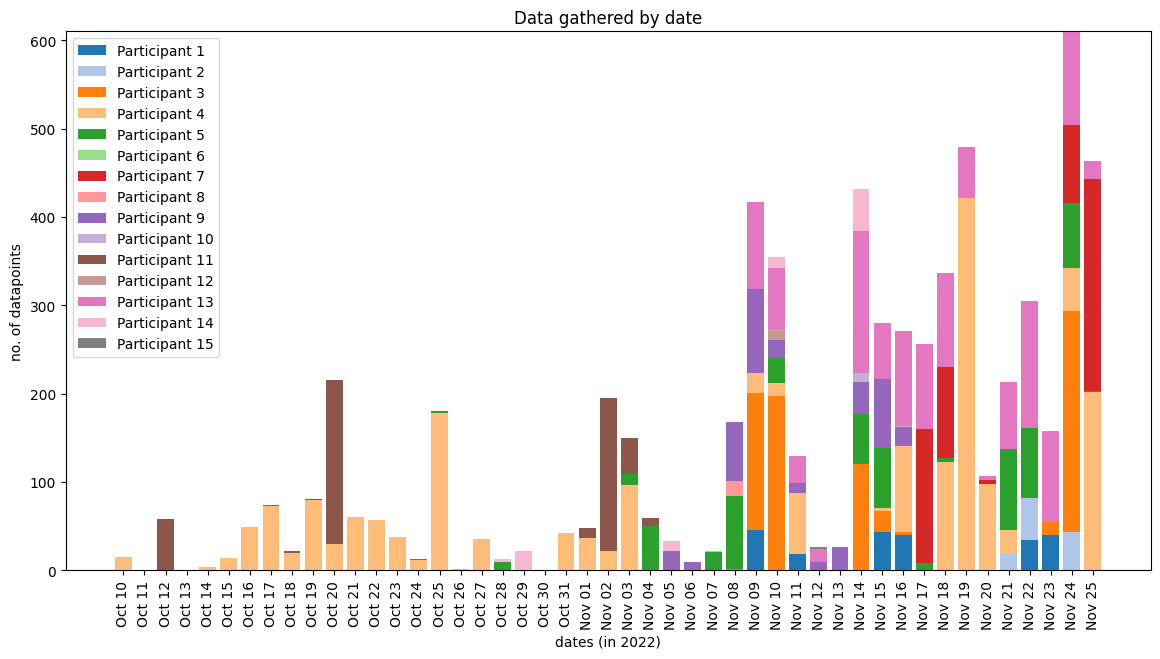
\includegraphics[scale=0.5]{chapters/methodology/graphics/data-gathered-dates.png}
  \caption{Data gathered from participants by date}
  \label{fig:data_by_date}
\end{figure}

\begin{figure}[htbp]
  \centering
  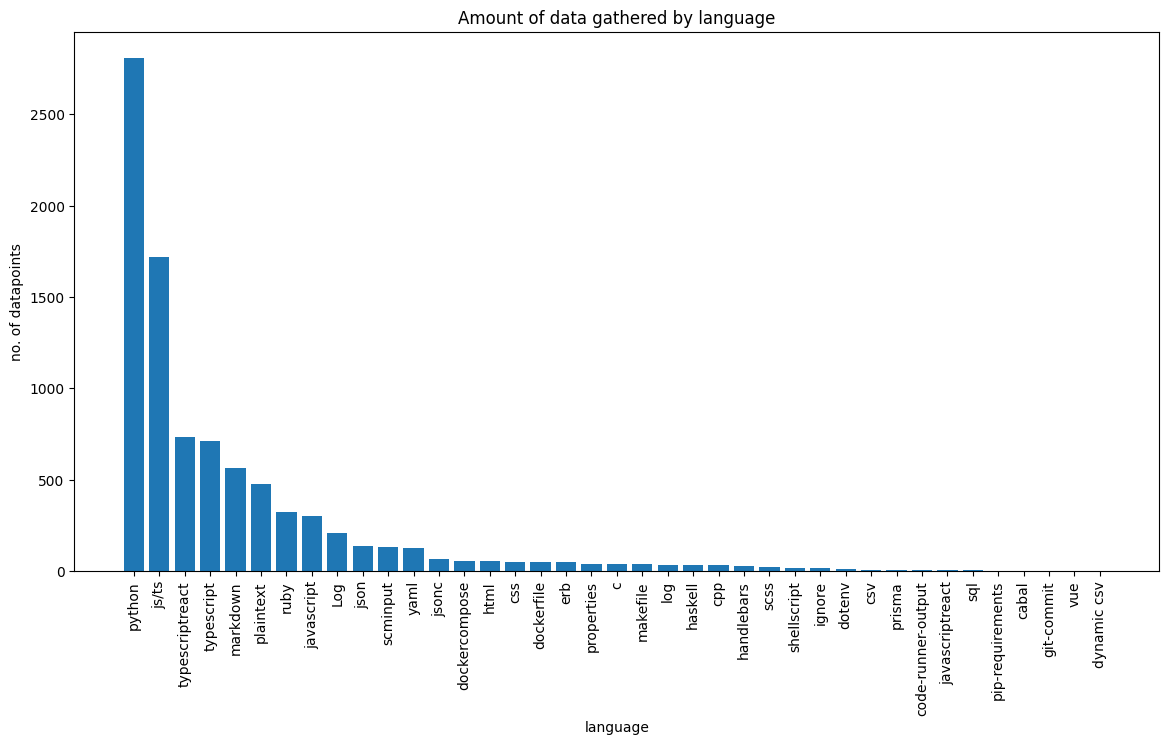
\includegraphics[scale=0.5]{chapters/results/graphics/languages-total.png}
  \caption{Amount of data gathered by language}
  \label{fig:data_by_langs}
\end{figure}

\section{Context}

% Released on	10/10/2022, 4:46:17 PM	
% Last updated	
% 10/21/2022, 2:29:27 PM

The data was gathered from different sources including: my acquaintances, students of my faculty reached directly and through the Facebook (a popular social media platform) group consociating them, as well as my former employers who volunteered to help. Attempts at gathering data from Reddit (a popular internet forum) users failed.

I offered certain rewards to encourage participation in the research project, which included a chocolate treat (inspired by the article of Feitelson et. al. \cite{Fei22DeveloperNames}), small amount donated to a charity and obviously an unrestricted access to the tool with all of its features in the current version. Research suggests that such external incentives are not particularly effective \cite{Coh19AltruisticSurvey, Bru11DifferentMotivations}, nevertheless it is my way of showing appreciation to the contributors without generating potential conflicts with the law. Redistributing digital goods, for instance, may be seen as a compelling way of rewarding, but it goes against EULAs (end user agreements \cite{EULA}). The charity incentive, however, may prove quite effective especially in the current times \cite{Forbes22Philanthropy}.

The tool is build on the top of Visual Studio Code \ref{fig:embedded_extension} (a popular IDE-like code editing software) due to its prevalence within the programming realm \cite{StackOverflow22Survey}. Furthermore, VS Code is easily extensible with the common TypeScript/JavaScript (JavaScript is pervasive in web development and TypeScript is basically typed JavaScript) framework and I have professional experience in building web applications.

In the end the \texttt{MIMUW-MB-TT} plugin was released on 10th October 2022 and last updated on 21st October 2022. The participants were instructed not to uninstall the plugin for one week at bare minimum or better at least for two weeks. As of 25th November 2022 the plugin was downloaded 33 times and 15 packages of user data has been gathered. The tactic of directly speaking to the faculty students and driving them to download my plugin by rewarded them with a chocolate seem to result with the most prominent source of participants in the study.

\begin{figure}[htbp]
  \centering
  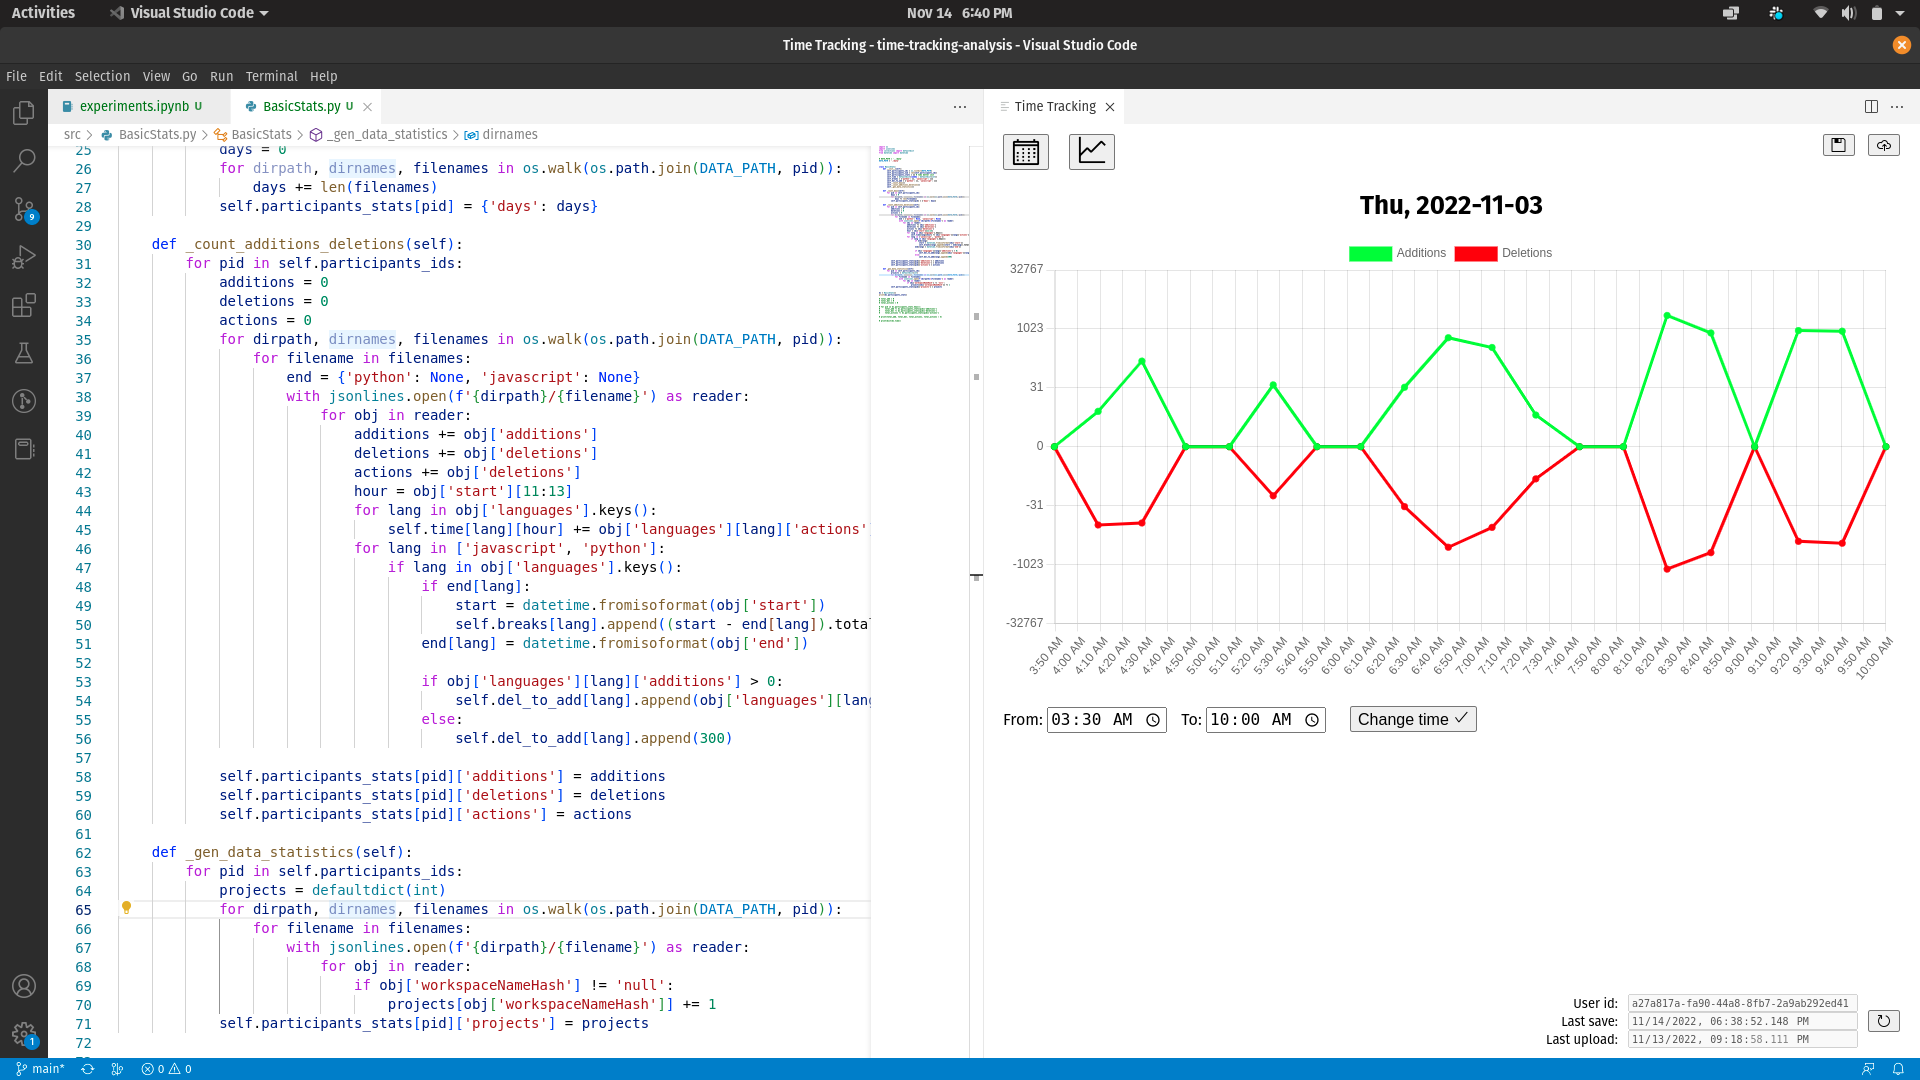
\includegraphics[scale=0.22]{chapters/methodology/graphics/extension-embedded.png}
  \caption{Extension embedded in Visual Studio Code}
  \label{fig:embedded_extension}
\end{figure}

\section{Data description}

The data is stored in the file system in the \texttt{JSON Lines} (\texttt{.jsonl}) \cite{JSONLines} format. It was popularized in recent years by OpenAI (a popular AI/ML company) in its GPT-3 API \cite{OpenAIGPT3}. Essentially files in this format are text files where each line (seperated by newline "\verb"\n"" characters) constitute a valid JSON value (that is why this format is sometimes also called \texttt{newline-delimited JSON}). In the particular case of my tool each of these JSON lines has a special designated type \ref{fig:event_type}.

\begin{figure}[ht]
    \centering
    \begin{verbatim}
{
  additions:                 INTEGER
  deletions:                 INTEGER
  actions:                   INTEGER
  start:                     STRING      // ISO 8601 date-time format
  end:                       STRING      // ISO 8601 date-time format
  workspaceNameHash:         STRING      // SHA-256 string or "null"
  languages: {               DICTIONARY
    [languageId: STRING]: {  DICTIONARY
      additions:             INTEGER
      deletions:             INTEGER
      actions:               INTEGER
    }
  }
}
\end{verbatim}

    \caption{The data type}
    \label{fig:event_type}
\end{figure}

Let me describe each of the fields of this structure:
\begin{description}
    \item[\texttt{additions}] say how many characters (chars) were added to the files opened in the editor within the time-frame determined by the fields \texttt{start} and \texttt{end};
    \item[\texttt{deletions}] say analogously to the \texttt{additions} field about the deleted chars;
    \item[\texttt{actions}] count how many actions were done on each file opened in the editor (one action may add or delete multiple chars);
    \item[\texttt{start}] means the start of the interval during which the record of the data was gathered;
    \item[\texttt{end}] is analogously to the \texttt{start} field the end of the interval;
    \item[\texttt{workspaceNameHash}] is the SHA256 \cite{NIST02SHS} hash of the workspace name in VSCode. It is done to secure the privacy of the research participants in the well established way (not to leak these names), but simultaneously to still be able to differentiate between the project names. If the workspace name does not exist, the value of \texttt{workspaceNameHash} is the string literal \texttt{"null"};
    \item[\texttt{languages}] is a dictionary that stores data separately for each (automatically recognized) programming language. It basically splits the fields \texttt{additions}, \texttt{deletions} and \texttt{actions} into contributions from each detected language.
\end{description}

% todo say that languages sums up to all additions and deletions (but not actions of course)

% Look in the similar papers.

% How did I encourage the people?

% Metion the papers on research motivations and the paper from the girl on naming the variables

% How much data was gathered?
% openai
\section{Premise}

I utilize the 30 seconds long intervals in order to simultaneously provide dense enough granularity and prevent user identification which may happen if intervals were too short. According to the article by Leinonen et. al. \cite{Lei17PreventIdentification} the identification stops being feasible when keystrokes are segregated into buckets of around 300 milliseconds (and more). My buckets (intervals) are much bigger and I do not save information about concrete keys pressed - I store only cumulative data (mainly added and deleting chars) within the given time-frame. Thus, I am convinced that this data is not straight-forwardly identifiable.

The data gathered in this way should give some insights into possible relations between programmers' activity (measured in chars added/deleted), used languages and the number of projects simultaneously worked on.

The user interface (UI), simply called the dashboard, is built with the research participants in mind. The purpose of the visualizations and the controls, that the dashboard provides, is to make the users more comfortable with the tool, to enhance trust in it and to potentially encourage them to use it regularly.

\section{Flow schema of the tool}

The data in the tool flows in several directions. User's action triggers changes in the source files. These changes cause the \texttt{TextDocumentChangeEvent} \cite{VSCodeAPI} events to be emitted. It is important to note here that the only changes that are tracked internally by VSCode are those associated with the files opened in the editor. Presumably, the reasons behind this mechanism are mainly performance ones. These events are then captured by the internal system. The internal system serves a few purposes (which are described in more detail in the subsection \ref{subsec:internal_system}). It is responsible for saving the data in the file system, compressing the data and sending it to the cloud storage (Dropbox in my case), as well as controlling the functions of the dashboard.

\begin{figure}[ht]
  \centering
  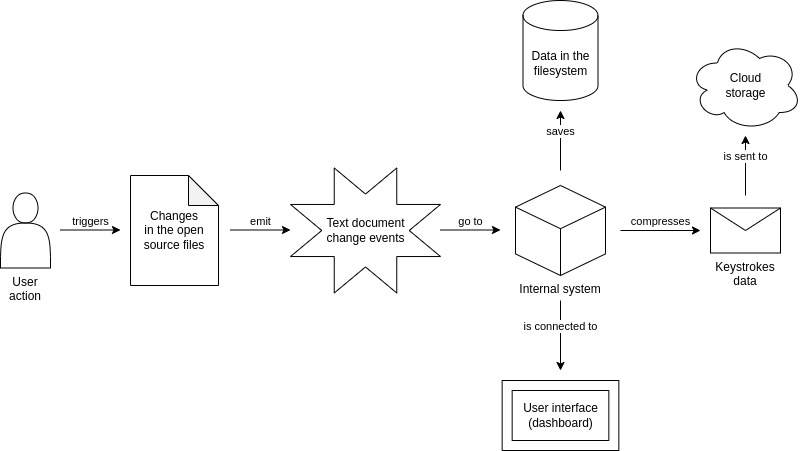
\includegraphics[scale=0.5]{chapters/methodology/graphics/coding-process-tracker.png}
  \caption{Flow schema of the tool}
\end{figure}

\section{Crucial elements of the \texttt{MIMUW-MB-TT} plugin}

\subsection{The internal system}\label{subsec:internal_system}

The main component of the internal system are the two buffers filled with the intervals. One of these buffers is the live buffer. The live buffer contains the data gathered lately. It is responsible for creating new intervals from the data that is coming from the user in the real time. The tool remembers to save the data in the file system in order to preserve it and not lose it all after potential crashes or closing the tool. After saving the data it is possible to remove some intervals from the live buffer in order to be aware of its size and not to allow it to get too big and clog the memory. The other of the buffers is the static buffer. It is responsible for loading the data from the file system in order for it to be then transferred to the dashboard. The user can request the data from the dashboard.

\begin{figure}[ht]
  \centering
  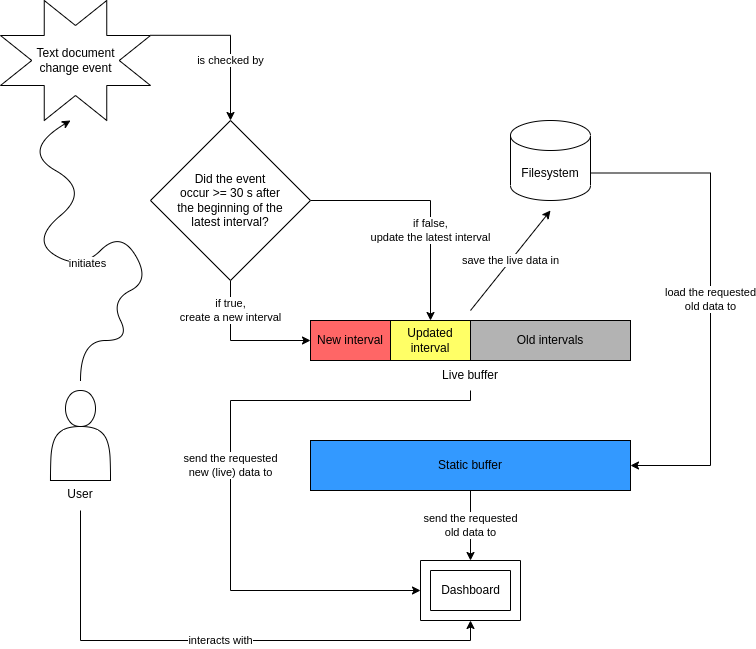
\includegraphics[scale=0.4]{chapters/methodology/graphics/internal-system.png}
  \caption{Internal system}
  \label{fig:internal_system}
\end{figure}

In order for for the intervals to be visualized they need to be normalized that is made to be of equal lengths. But the raw data consists of the intervals of varying lengths that is of length at most 30 seconds. I need to adjust them to be even-sized. Normalization recognizes also that the intervals need to stick to each other, however in the raw data there may exist breaks, since there are situations where for some time a user may be inactive. So essentially I can treat the time spaces that are not covered by the data as intervals with zero keystrokes. Then by interpreting this data such way I can proceed with interpolation (as shown in the example \ref{fig:internal_system}). Let me imagine that I split the requested time space into intervals of equal length and then I check if they intersect with the intervals from the real data. The amount of keystrokes that the new interval receives is proportional to the relative size of the intersection to the length of the whole row interval.
% So it's about you looking at the example from the figure if the intersection constitutes 30\% of the row interval then then we take into account 30\% of keystrokes from this row interval to the new interval of equivalent.
The total number of keystrokes associated with this new interval is calculated by summing all of the keystrokes associated with all the intersections from the different row intervals.

\begin{figure}[htbp]
  \centering
  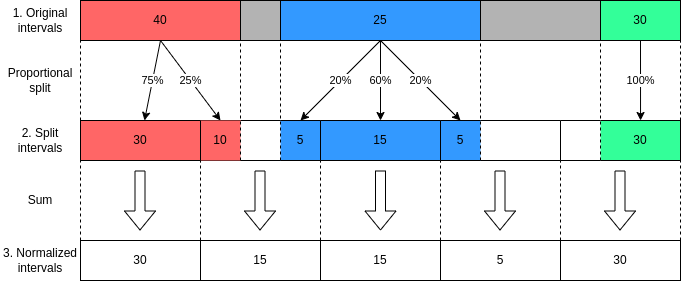
\includegraphics[scale=0.5]{chapters/methodology/graphics/normalization.png}
  \caption{An intervals normalization example}
  \label{fig:normalization_example}
\end{figure}

\subsection{Dashboard (UI)}

The dashboard constitutes the user interface that a user can use to view various statistics across different time periods. It is possible through switching modes. The first mode is called the live view \ref{fig:live_view}. In this view the user is able to view the latest data. Hovering over the data points on the plot (green or red dots on the line) reveals a tooltip containing more details (mainly the exact numerical values of the respected data point). The user can also adjust the time gauge to explore the data in the different time periods (last 10, 30 or 60 minutes from the current time). Moreover, he is provided with the Calendar view \ref{fig:calendar_view}. It is utilized to explore the data from previous days. After selecting the current day the user can also adjust the time period by using the aforementioned gauges. The parameters of the plot are adjusted automatically in order for the plot to be clearly visible to the user. This means to be not too convoluted and not too cluttered. The dashboard is connected with the live and static buffers and depending on the view the data is loaded from the live buffer or from the static buffer (that is indirectly from the file system). It is possible through the day view \ref{fig:day_view} that is accessible by selecting a day in the calendar view.

Users are enabled to save and upload the data manually by clicking on the buttons in the upper-right corner of either of the views. Since the quota of API calls to Dropbox servers is limited with my subscription plan, I have implemented a cooldown period on subsequent manual uploads to conserve the available API invocations.

\begin{figure}[htbp]
  \centering
  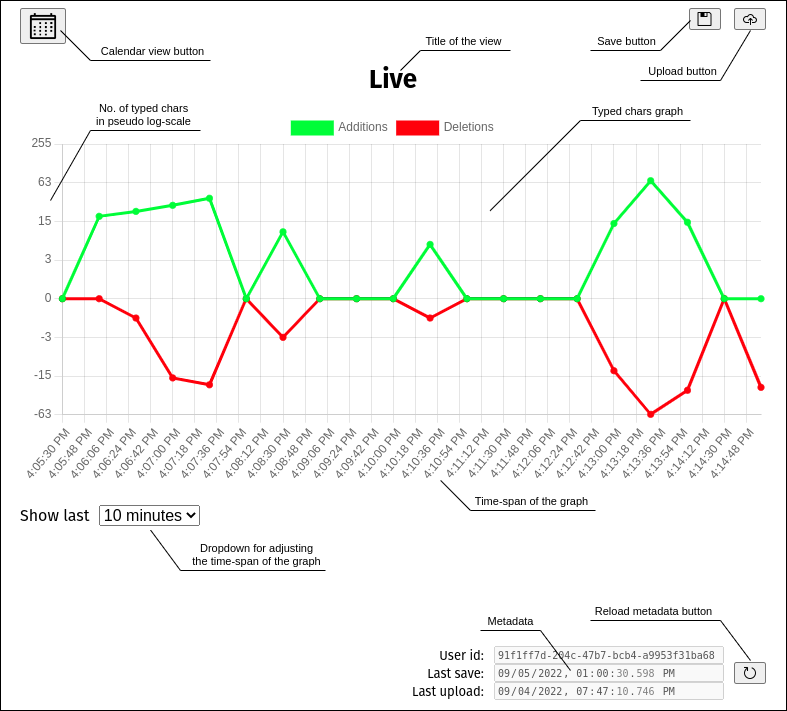
\includegraphics[scale=0.4]{chapters/methodology/graphics/live-view.png}
  \caption{Live view of the dashboard}
  \label{fig:live_view}
\end{figure}

\begin{figure}[htbp]
  \centering
  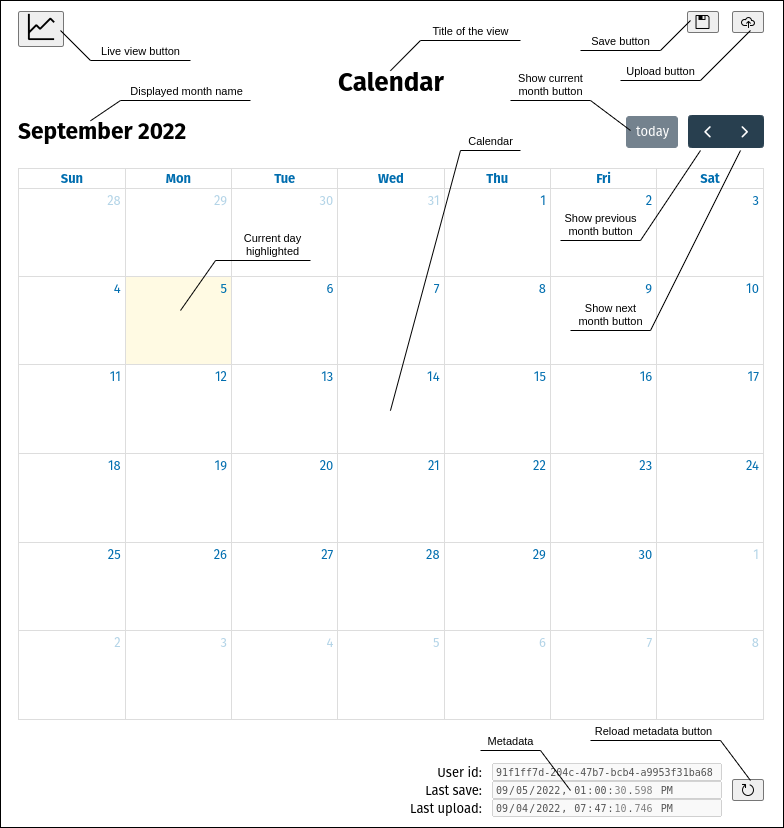
\includegraphics[scale=0.4]{chapters/methodology/graphics/calendar-view.png}
  \caption{Calendar view of the dashboard}
  \label{fig:calendar_view}
\end{figure}

\begin{figure}[htbp]
  \centering
  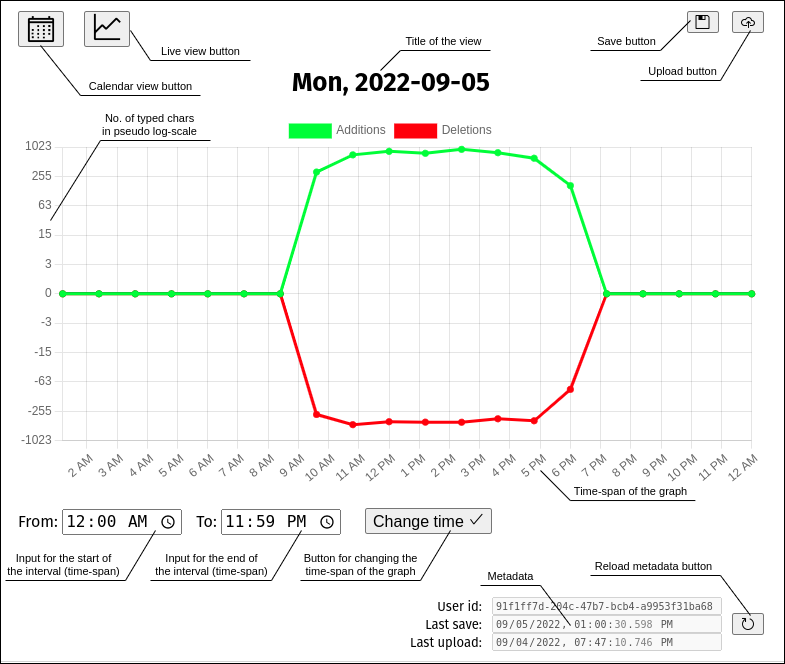
\includegraphics[scale=0.4]{chapters/methodology/graphics/day-view.png}
  \caption{Day view of the dashboard}
  \label{fig:day_view}
\end{figure}

\section{Research questions}

\subsection{What are the activity patters of programmers during the day?}

I examine if the programmers of different languages remain active during the day and night. It is achieved by analyzing data points with regards to their timestamps and programming languages used. Additionally, I compute the performance metric measured by the average number of actions per data point to hypothesize about performance fluctuations with regards to moving time. This statistic also takes into account the programming language to search for potential divergence in activity patters between people using different languages.

\subsection{How do programmers take breaks during the day?}

Programmers need breaks between coding to read the code, study documentation, complete various professional tasks or just to have lunch. To analyze these breaks, I compute the lengths of all the recorded spaces between data points within a day (omitting the breaks taken between different days). This way it becomes possible to bin the data about breaks and compose a histogram to observe the frequency of shorter and longer breaks for programmers. Again, the programming language is also taken into account here.

\subsection{What are the proportions of code added to code deleted?}

Programmers during coding may not only add the new code, but also delete the old one and replace it. I study the characteristics of this behavior by analyzing the ratio of the number of deletions to the number of additions. Small values of this ratio (below 100\%) indicate the increase in the code base, while higher values (over 100\%) point to the code being mostly removed. The ratio is calculated separately per data point and per day to find out if the statistical trends hold under diverse granularity levels. Similar check is done on the basis of the difference in the programming language used.

\subsection{How many projects do programmers work on?}

It is quite common for programmers to work on multiple projects in parallel especially since they may constitute the basis of a larger venture. I examine what is the usual number of projects that the programmers work on during the day and overall. Additionally, I check how frequent it is to switch between different projects within one day.

% \subsection{How many languages do programmers use?}

% I can see if the programmers work on many languages and what configurations.

\subsection{How does the data change in relation to the day of the week?}

It is expected that programmers' activity decreases on the weekend. I validate these claims by comparing the number of data points and actions generated in distinct days of the week. Performance (measured as the average number of actions per data point) is also calculated with this regard to search for potential disparity in programmers' performance between weekdays and the weekend days.

% I will do that by searching for time periods of particularly increased or decreased activity. I will observe that frequency of extreme points (especially peaks) in the plots. This way I can make hypotheses about the actual real actions of programmers. For instance in the Version Control systems merging code may result in high numbers of additions or deletions. Such suspicious peaks of activity may provide evidence to particular actions.


\chapter{Results}\label{ch:results}

% stereotypical differences in programmers depending on programming languages - move it elsewhere

% CSS and HTML are not technically programming languages - move it elsewhere

% \textcolor{red}{TODO!!! day vis repr}

\section{Activity}

On the figure \ref{fig:activity_by_hour}, the activity of programmers by hour is presented. It is measured in two ways: by counting the data points generated in distinct hours, and by summing the actions within these data points. I remind that \texttt{actions} is an attribute of a data point \ref{sec:data_description} and here I sum these attributes of multiple data points. In both cases of measurement the \texttt{start} timestamp determines the hour bucket where a data point or an action falls under. Timezone from the timestamps is ignored here and in analogous graphs later. Thus, for instance, two programmers working at 10:00 in Warsaw and at 10:00 in San Francisco on the same day would contribute to the same hour bucket. On the graph it is clearly observed in both of the measurement ways that most of the activity happens in the afternoon and that the work almost completely ceases in the middle of the night and around dawn.

\begin{figure}[htbp]
  \centering
  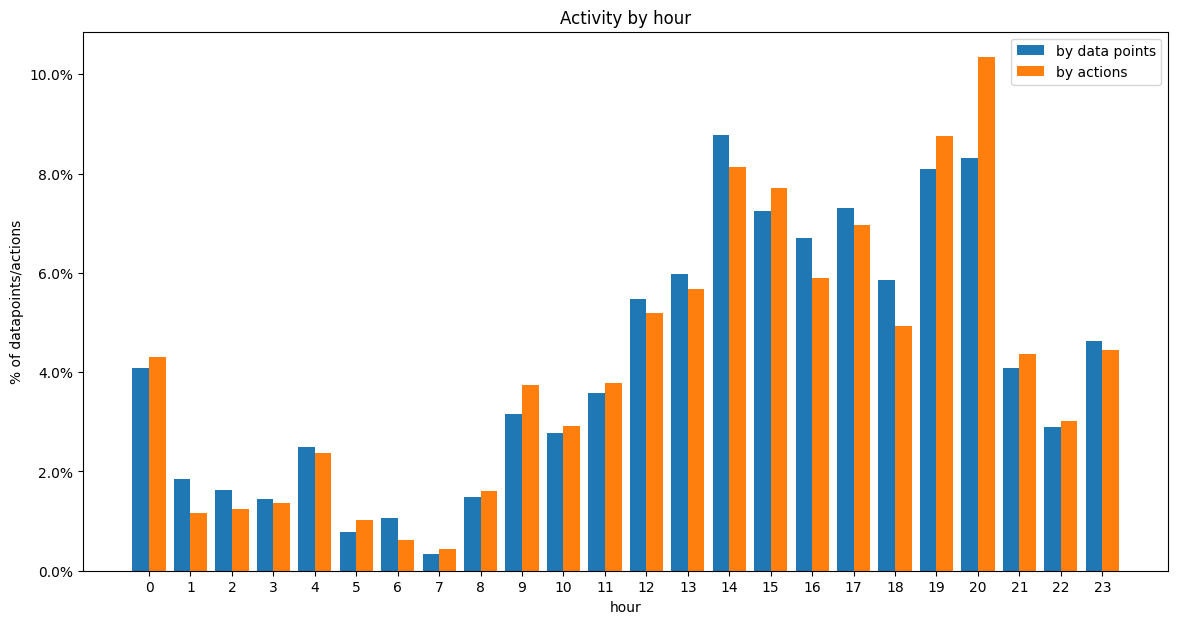
\includegraphics[scale=0.5]{chapters/results/graphics/activity-by-hour.png}
  \caption{Comparison of activity by hour with regards to data points and actions}
  \label{fig:activity_by_hour}
\end{figure}

Similar observations can be made by examining the activity graph with respect to different programming languages \ref{fig:activity_by_hour_langs}. The noticeable difference may be that for JS/TS developers the activity is strongly concentrated in the afternoon where for Python developers some activity is also observed during the night.

\begin{figure}[htbp]
  \centering
  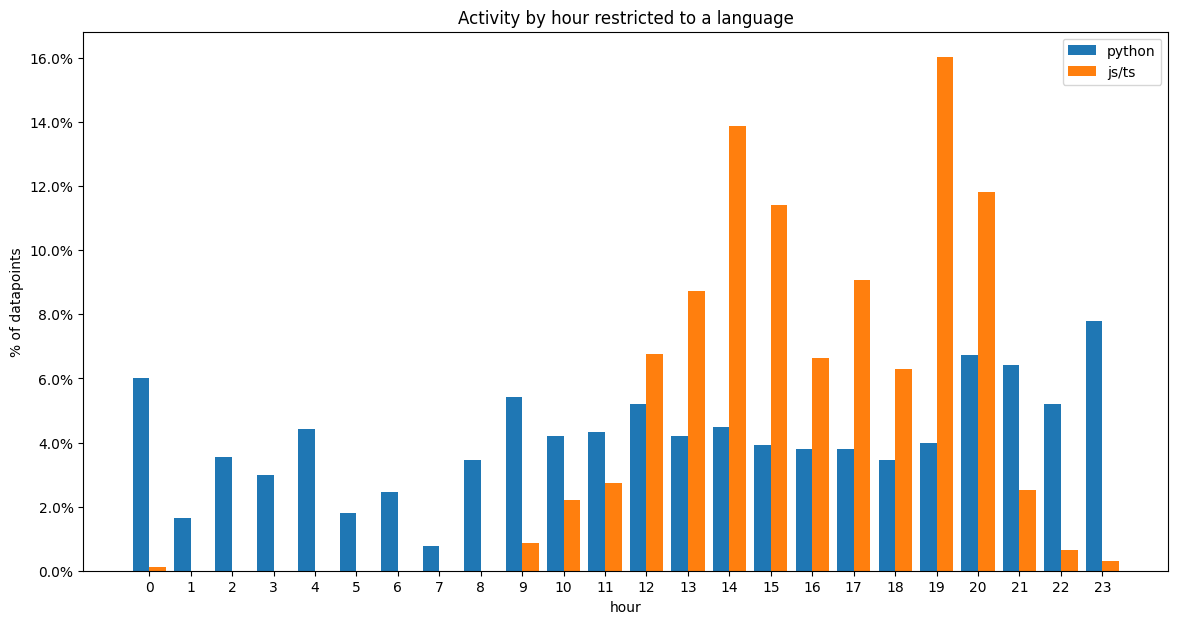
\includegraphics[scale=0.5]{chapters/results/graphics/activity-by-hour-langs.png}
  \caption{Comparison of activity by hour restricted to a language}
  \label{fig:activity_by_hour_langs}
\end{figure}

When it comes to performance measured as the average number of actions per data point, it remains relatively stable \ref{fig:performance_by_hour} with visible dips around the end of the standard working day (i.e. between 4 and 6 pm) and at night. Perceived anomalous surges during that period (i.e. at 12 and 5 am) occurred arguably due to smaller samples of data gathered at those time slots.

\begin{figure}[htbp]
  \centering
  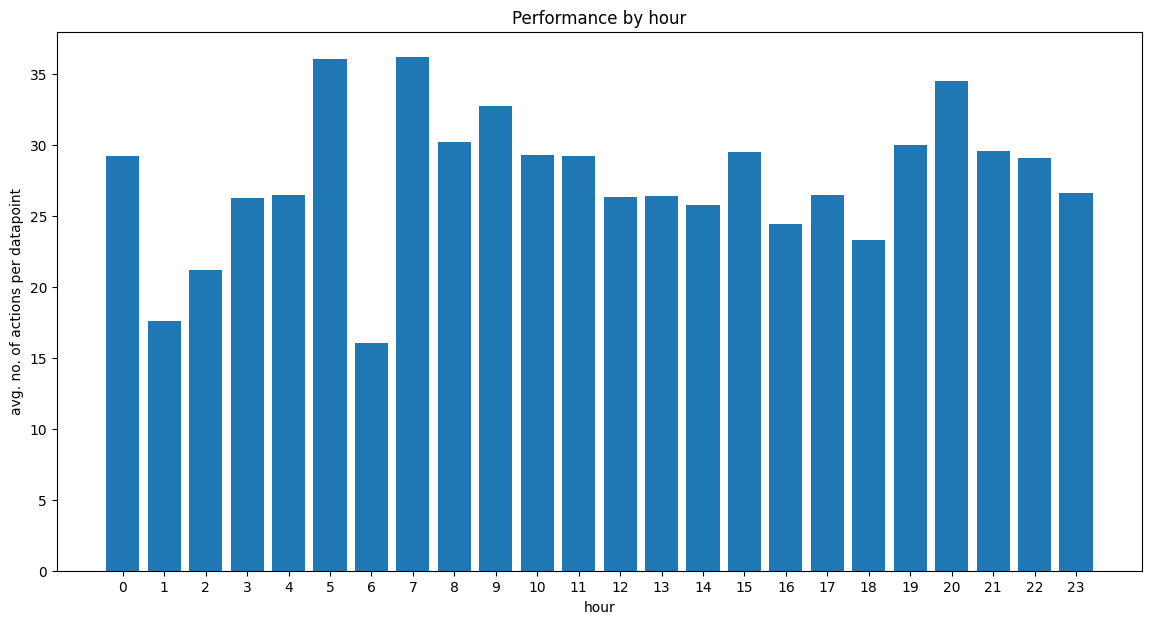
\includegraphics[scale=0.5]{chapters/results/graphics/performance-by-hour.png}
  \caption{Performance by hour}
  \label{fig:performance_by_hour}
\end{figure}

Such a trend is less clearly visible when restricted to Python and JS/TS languages \ref{fig:performance_by_hour_langs}, but this may be due to the fact that much less data was gathered at night and in the case of JS/TS even none in the majority of night hours. Comparing the results between the languages, it is noticeable that the performance metric for JS/TS developers is generally higher than for the Python ones (ignoring the night period).

\begin{figure}[htbp]
  \centering
  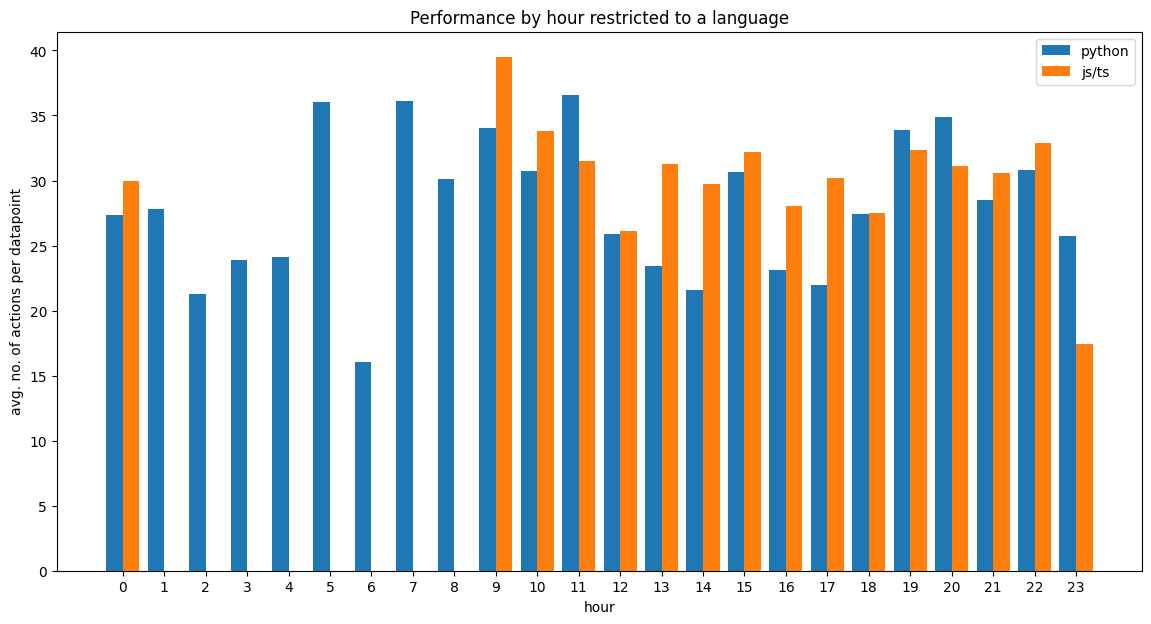
\includegraphics[scale=0.5]{chapters/results/graphics/performance-by-hour-langs.png}
  \caption{Performance by hour restricted to a language}
  \label{fig:performance_by_hour_langs}
\end{figure}

\section{Breaks}

There is no observed striking disparity between programmers of different languages and overall \ref{fig:breaks}. Understandably, the longest breaks are much less frequent than the shorter ones. Nevertheless, it is not the shortest breaks that are the most frequent, but the middle length breaks of about 30 seconds.

\begin{figure}[htbp]
  \centering
  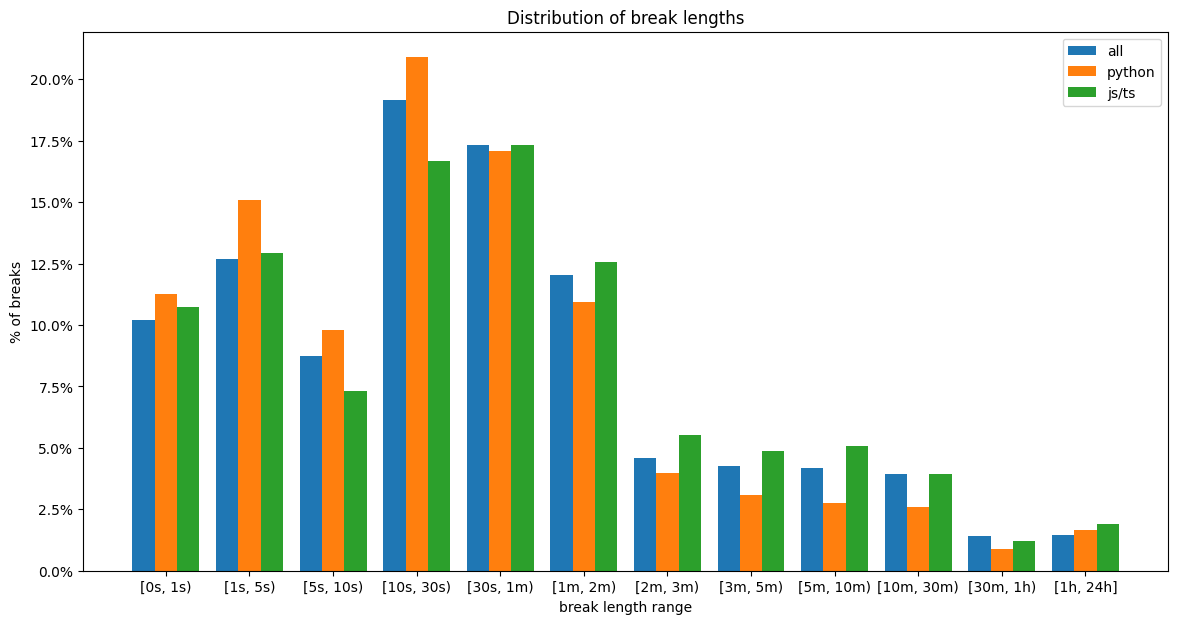
\includegraphics[scale=0.5]{chapters/results/graphics/breaks.png}
  \caption{Distribution of break lengths overall and restricted to a language}
  \label{fig:breaks}
\end{figure}

\section{Deletions to additions}

For both granularities (per data point and per day), there is a trend of decreasing frequency of ratios with the increase of deletions relative to additions \ref{fig:del_to_add}. There are two apparent exceptions from this tendency. The days with a slightly higher number of deletions to additions are much more frequent than in the case of data points. Apart from that, quite common are occurrences where the number of deletions is much higher than additions (signified by the last bars on the right of the plots).

\begin{figure}[htbp]
  \centering
  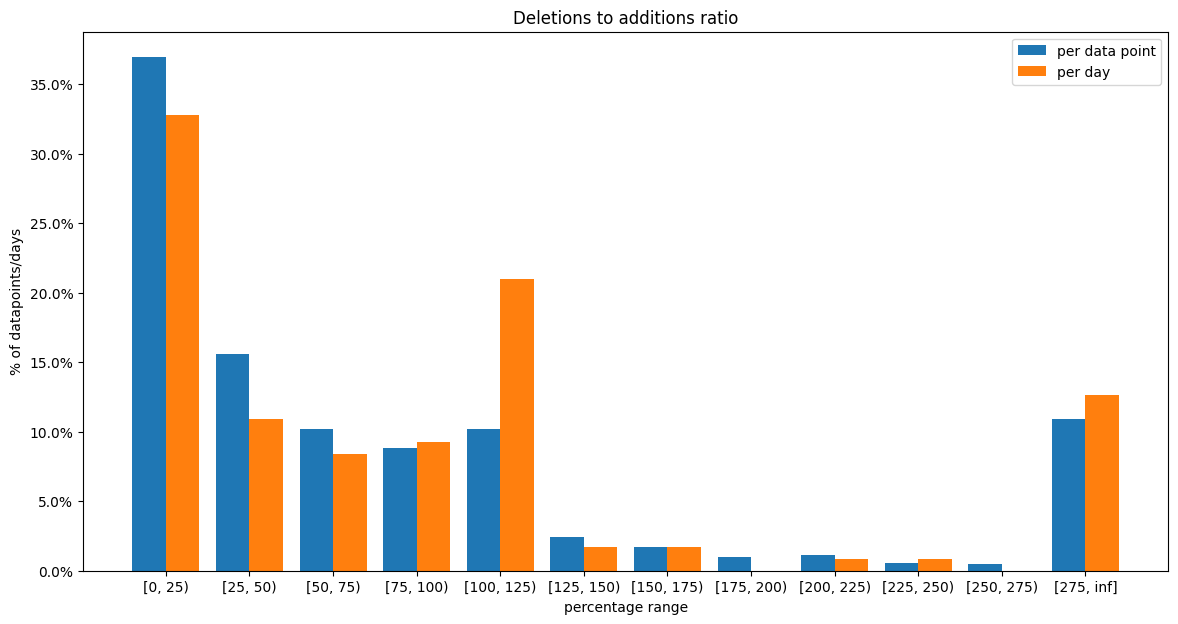
\includegraphics[scale=0.5]{chapters/results/graphics/del-to-add.png}
  \caption{Deletions to additions with regards to data points and days}
  \label{fig:del_to_add}
\end{figure}

There are no particular differences between Python and JS/TS developers with regards to the regarded ratio. One thing that is visible is the higher occurrence of the data points with lower ratio (i.e. more additions) in the case of Python comparing to JS/TS.

\begin{figure}[htbp]
  \centering
  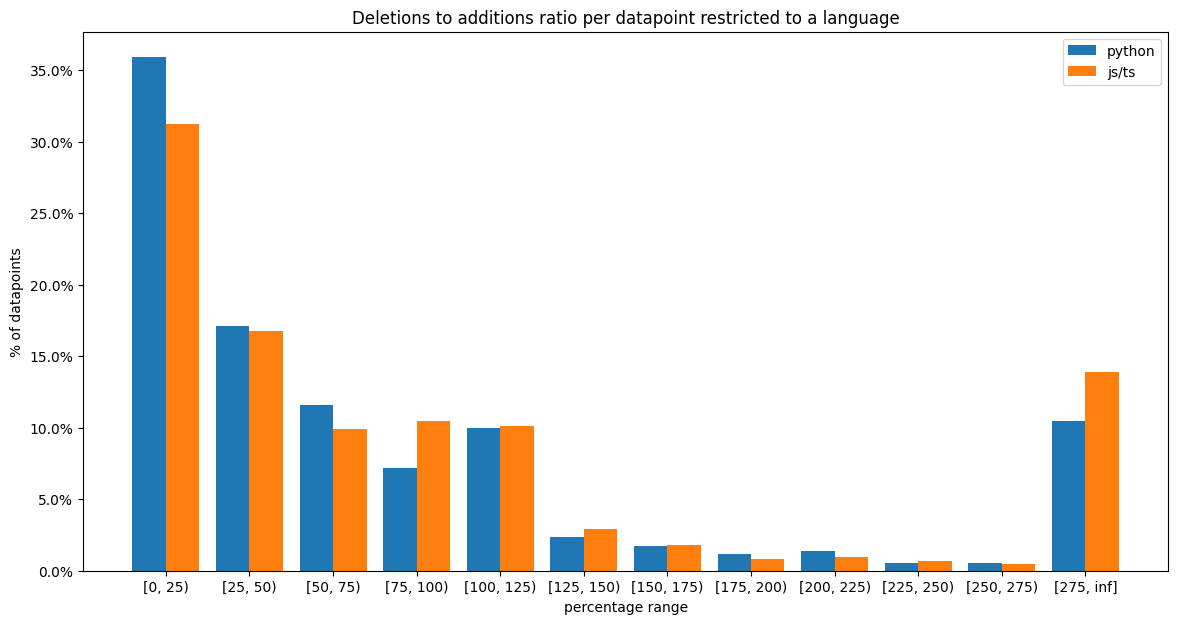
\includegraphics[scale=0.5]{chapters/results/graphics/del-to-add-langs.png}
  \caption{Deletions to additions restricted to a language}
  \label{fig:del_to_add_langs}
\end{figure}

\section{The number of projects}

In the vast majority of cases a programmer works on one project per day according to the data \ref{fig:projects_per_day}. Cases with 5 or more projects were not recorded. Situations were no projects were recorded during the day (i.e. a user in VS Code works outside the named workspace) remain very scarce.

\begin{figure}[htbp]
  \centering
  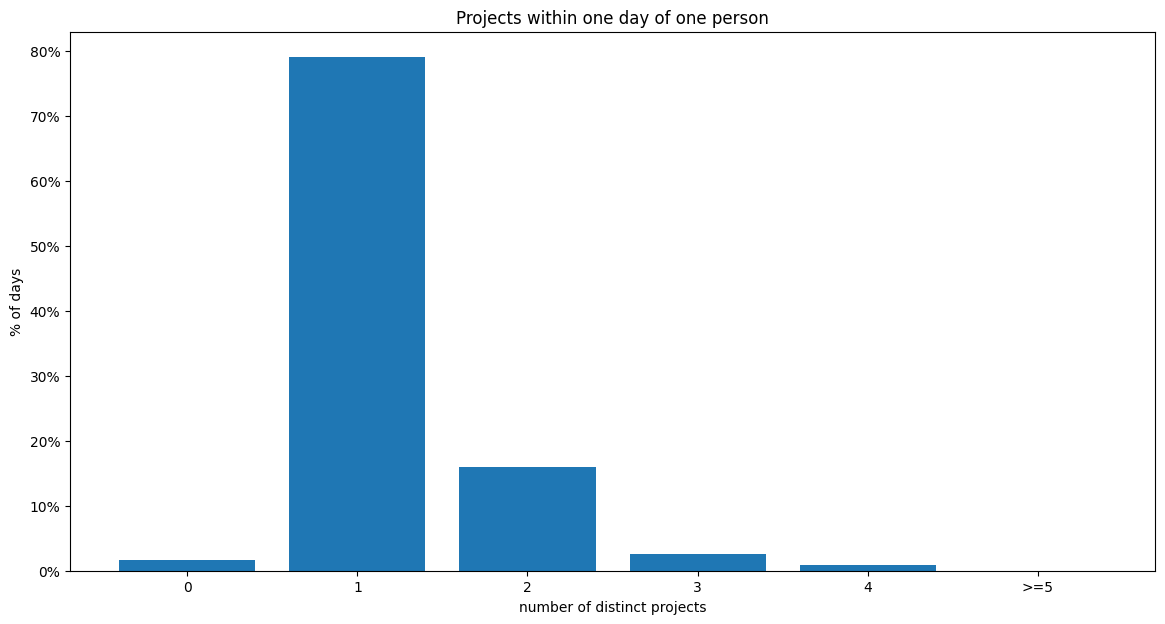
\includegraphics[scale=0.5]{chapters/results/graphics/projects-day.png}
  \caption{Number of projects within one day of a programmer}
  \label{fig:projects_per_day}
\end{figure}

A similar picture is observed even when considering all the projects of one person within the time frame of my research \ref{fig:projects_per_person}. Cases with 6 or more recorded projects per person were uncommon and most oscillated between 1 and 3.

\begin{figure}[htbp]
  \centering
  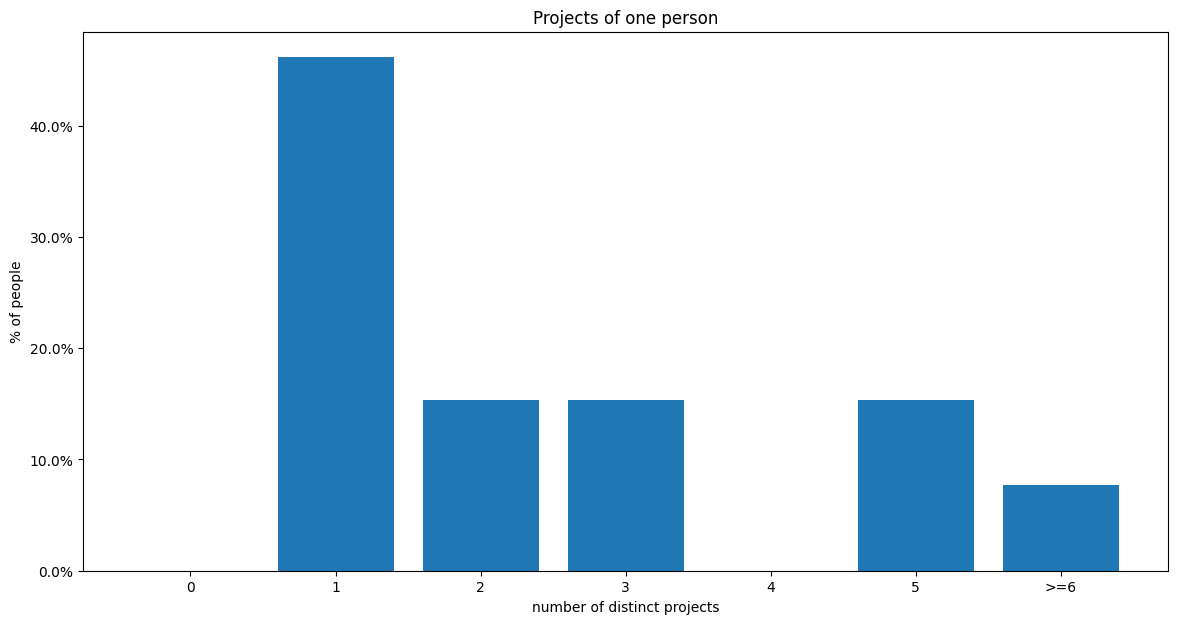
\includegraphics[scale=0.5]{chapters/results/graphics/projects-one-person.png}
  \caption{Number of programmer's projects}
  \label{fig:projects_per_person}
\end{figure}

It turns out that according to the data it is also uncommon to switch projects during the working day \ref{fig:projects_switching_per_day}. During the staggering most of the days developers did not switch the project even once.

\begin{figure}[htbp]
  \centering
  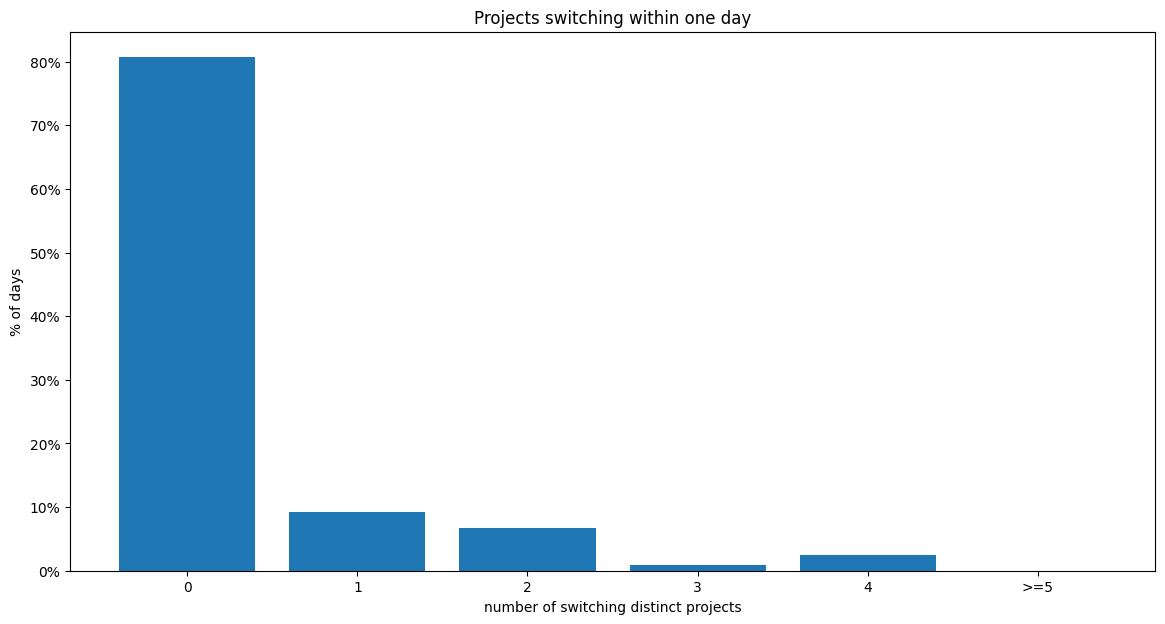
\includegraphics[scale=0.5]{chapters/results/graphics/projects-switching-day.png}
  \caption{Number of projects switching within one day of a programmer}
  \label{fig:projects_switching_per_day}
\end{figure}

% \section{Mixing languages}
\section{Per weekday differences}

The activity peaks in the middle of the week and decreases on Friday, only to slump during the weekend \ref{fig:weekday_activity}. Regardless of the measurement method (by counting data points or summing up actions), the aforementioned trends seem consistent.

\begin{figure}[htbp]
  \centering
  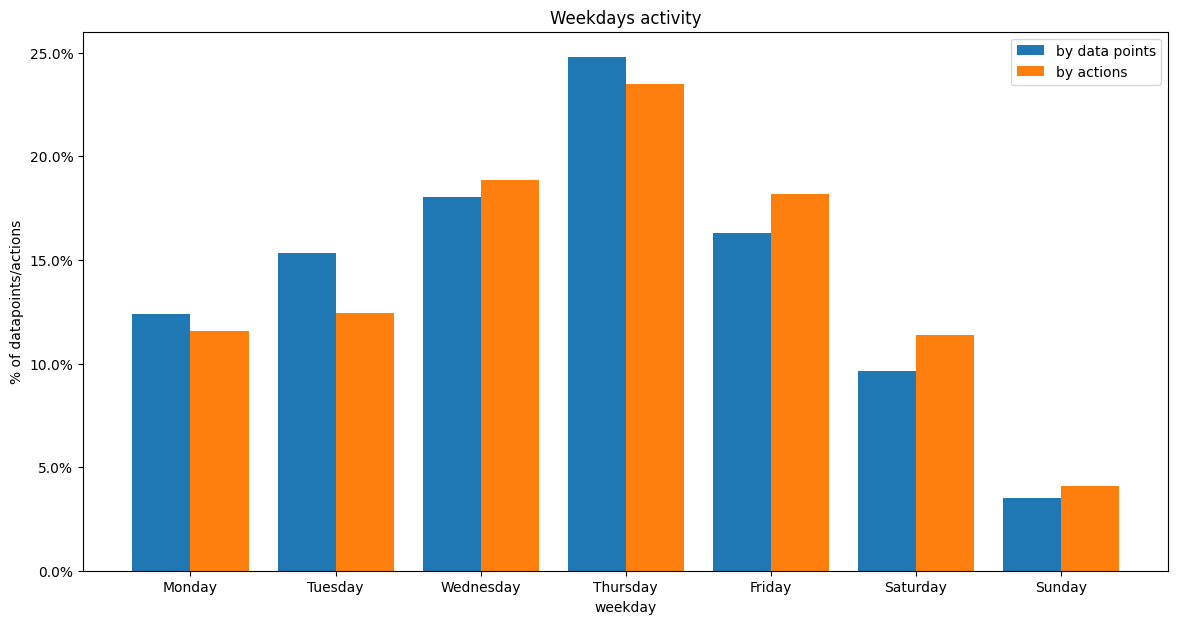
\includegraphics[scale=0.5]{chapters/results/graphics/activity-by-weekday.png}
  \caption{Activity per weekday with regards to data points and actions}
  \label{fig:weekday_activity}
\end{figure}

Analysis of performance did not give any conclusive results with them appearing relatively stable \ref{fig:weekday_performance}.

\begin{figure}[htbp]
  \centering
  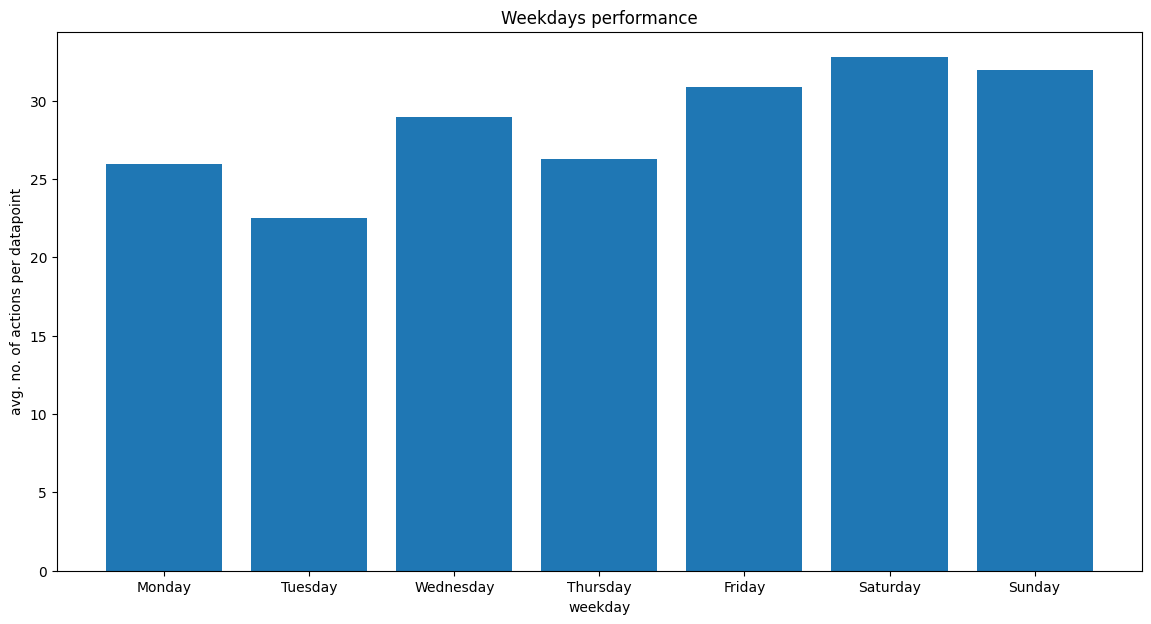
\includegraphics[scale=0.5]{chapters/results/graphics/weekdays-performance.png}
  \caption{Performance per weekday}
  \label{fig:weekday_performance}
\end{figure}


\chapter{Discussion}\label{ch:discussion}

\section{Revisiting results}

Analysis of the data gathered by the \texttt{MIMUW-MB-TT} plugin sheds some light onto the characteristics of programmers' working day.

Visualizations of a working day of a programmer give potentially valuable insights into the programming process. The developer can introspect and measure his performance. His employer is able to more accurately assess the productivity and potentially provide the assistance where it is needed the most.

Activity analysis shows that understandably most of the work concentrates in the afternoon, but with a notable portion of it done in the evening. Similar patterns emerge when analysing the data from programmers of Python and JS/TS separately. Nevertheless, no sound evidence towards difference of chronotypes between programmers of different languages were discovered.

Breaks analysis unsurprisingly concludes that longer breaks are less frequent that shorter ones and this observation holds for different programming languages and overall. The reason why middle length breaks are more frequent than the shortest ones may just be related to the method of measurement with a break considered as a time space between two data points. Let me remind here that one data point holds information of at most 30 seconds.

Analysis of the ratio of deletions to additions shows that it is more common to add code than to delete it and this trend stays true regardless of the programming language used.

The number of projects per person is observed as at most just a few. Moreover, frequent switching between different projects was not observed.

The data supports the common knowledge that activity dips on weekends. Additionally, it decreases even earlier on Friday which was observed also by Robinson \cite{Rob17LangsUsedAtNight}.

\section{Threats to validity}

\subsection{Doubts about data gathered}

I gathered the data from 15 programmers. This number comes from counting the data packages I have received throughout the study. I assume that each of them comes from a different person, although it is theoretically possible that one person uses the \texttt{MIMUW-MB-TT} plugin on separate workstations, thus is counted multiple times. From my personal talks with the participants, I assess the probability of such occurrences as low.

Although the participants were instructed to use the plugin for at least two weeks, the number of downloads significantly surpass the number of data packages (a minority of them were test downloads by me) and even within the packages there are differences of size between them. Because of that, some participants may influence the final results stronger than the rest.

\subsection{Questions about participants in the study}

Apart from the number of participants, it is important to remember they were not chosen uniformly from the whole community of programmers. Most of them came from the MIMUW faculty as student and it may significantly incluence the final results.

\subsection{\texttt{MIMUW-MB-TT} plugin shortcomings}

Due to the technical obstacles, the plugin does not save the data in the file system right before closing the VS Code window. It just saves the data on 2 minutes interval, so it is possible to lose the data gathered right before closing the IDE.

Additionally, there exist an exploit related to project switching. Since \texttt{workspaceNameHash} relates to the last workspace name recorded for a data point, it is theoretically possible to work within 30 second period on different projects and the system would store such an event as working on just one. This would, however, involve quite a deep knowledge of the plugin and rather unnatural way of typing, so I deem the risk of this exploit influencing the gathered data as minimal.

Apart from that, the plugin allows a situation where \texttt{start} and \texttt{end} are equal for a data point. While this does not constitute a bug by itself, it creates potential confusion and inconvenience when analyzing the gathered data.

\chapter{Conclusions and future work}

% Getting more data
% Publishing the tool

% Say that it's possible to ask why some things happen (annotations)

\chapter{Data and code availability}\label{ch:publishing}

In order to streamline my processes and make them more appealing to the public and to mitigate the risk of de-anonymization \cite{Nar08DeAnon}, a part of the agreement was not to publish any keystroke data of my testing subjects. At GitHub I have published the source code of \href{https://github.com/goalon/time-tracking}{my plugin}, the source code available for \href{https://github.com/goalon/time-tracking-analysis}{data analysis} and the Latex source code of \href{https://github.com/goalon/masters-thesis}{this thesis}. Anyone also can download my plugin directly from VS Code or at \href{https://marketplace.visualstudio.com/items?itemName=MateuszBajorekMIMUW.mimuw-mb-tt-time-tracking}{Visual Studio Marketplace} \ref{fig:marketplace}.

\begin{figure}[htbp]
  \centering
  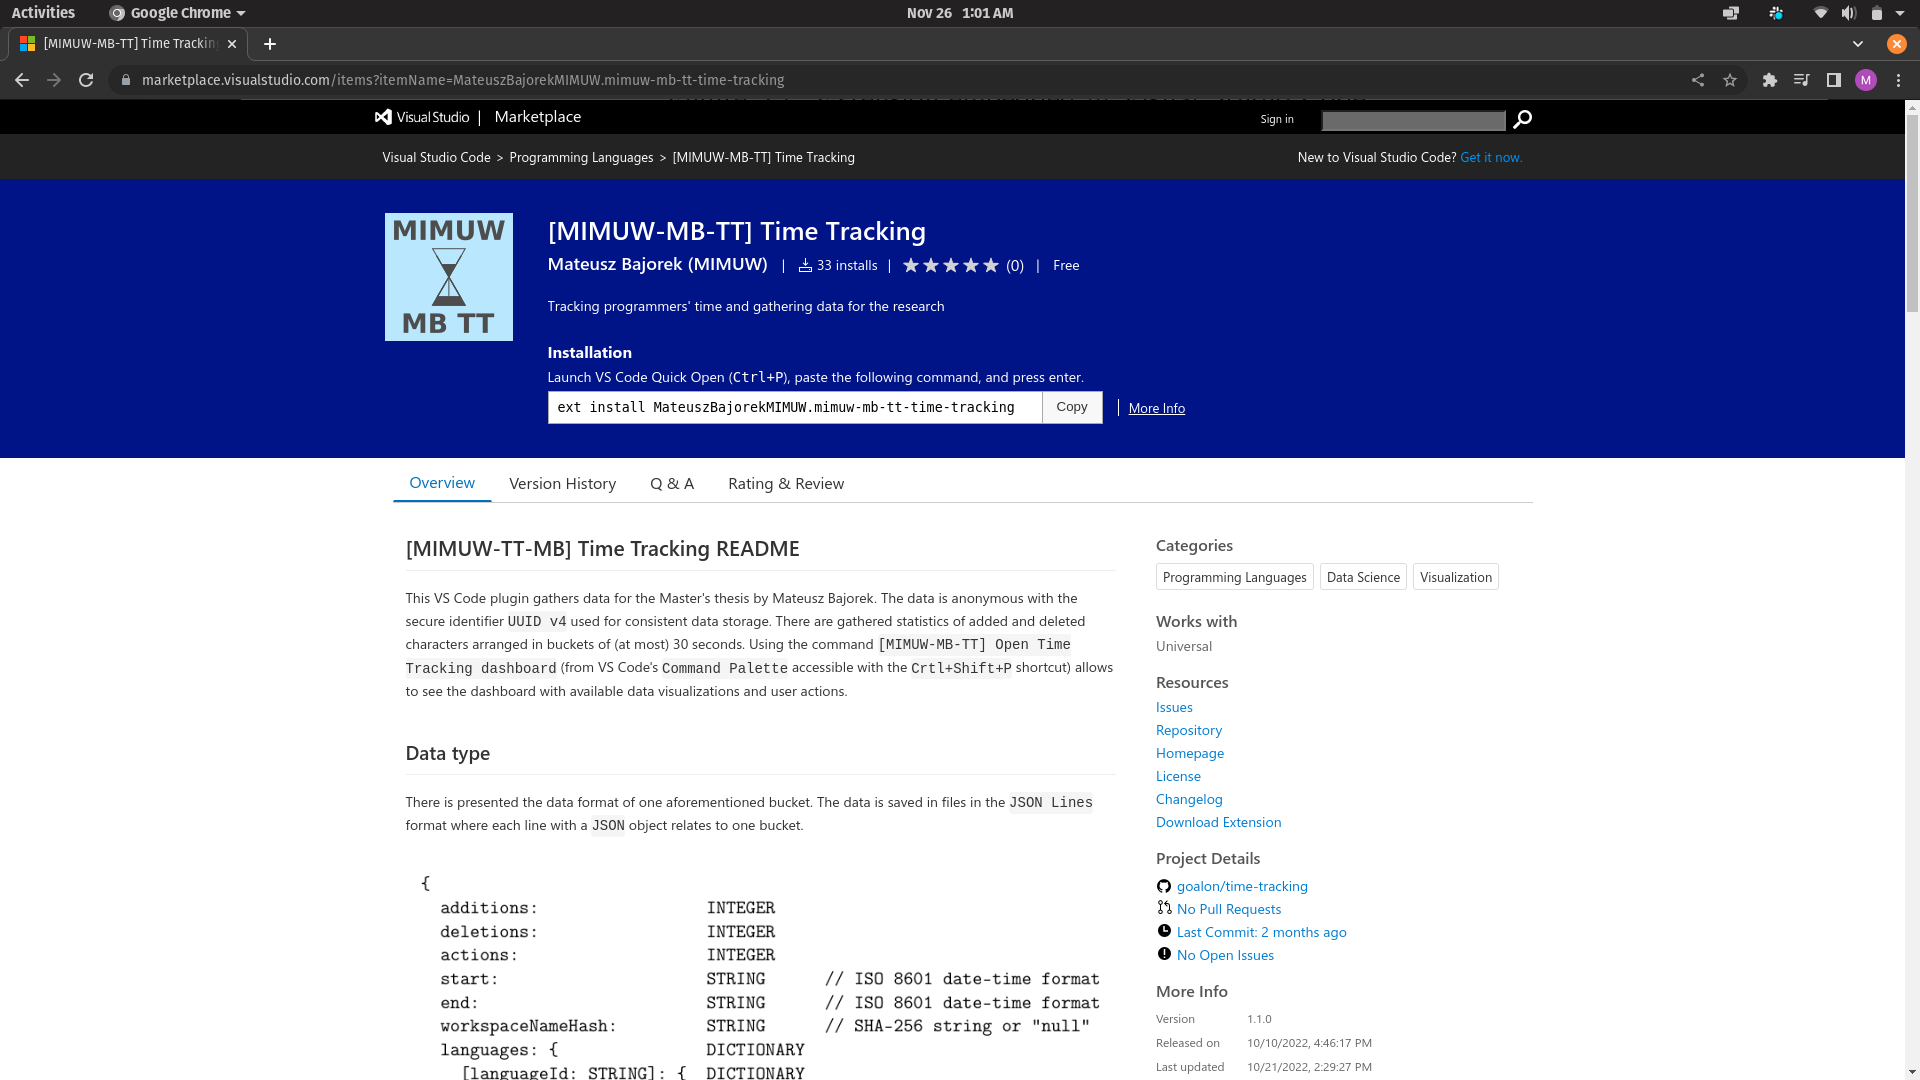
\includegraphics[scale=0.22]{chapters/availability/graphics/marketplace.png}
  \caption{\textit{MIMUW-MB-TT} plugin in the VS Marketplace (as of 26 Nov 2022)}
  \label{fig:marketplace}
\end{figure}


\appendix

\begin{thebibliography}{99}
\addcontentsline{toc}{chapter}{Bibliography}

\bibitem[1]{Rep02CircadianTiming} Steven M. Reppert, and David R. Weaver. 2002. \textit{Coordination of circadian timing in mammals}. Nature 418, 935–941, doi: \href{https://doi.org/10.1038/nature00965}{10.1038/nature00965}.

\bibitem[2]{Roe03Chronotypes} Till Roenneberg, Anna Wirz-Justice, and Martha Merrow. 2003. \textit{Life between Clocks: Daily Temporal Patterns of Human Chronotypes}. Journal of Biological Rhythms, 18(1), pp. 80–90, doi: \href{https://doi.org/10.1177/0748730402239679}{10.1177/0748730402239679}.

\bibitem[3]{Sto21ProgrammersDo} Dale Stokdyk. 2021. \textit{What Do Programmers Do, Anyway?} Southern New Hampshire University, url: \url{https://www.snhu.edu/about-us/newsroom/stem/what-do-programmers-do}.

\bibitem[4]{Fed21TimeTracking} Tony Fedorenko. 2021. \textit{Time Tracking in Software Development}. Mad Devs, url: \url{https://maddevs.io/customer-university/time-tracking-in-software-development/}.

\bibitem[5]{Gro21SDMHistory} Growin. 2021. \textit{A Brief History of Software Development Methodologies}. Growin Blog, url: \url{https://www.growin.com/blog/history-of-software-development-methodologies/}.

\bibitem[6]{Tho05} Richard C. Thomas, Amela Karahasanovic, and Gregor E. Kennedy. 2005. \textit{An investigation into keystroke latency metrics as an indicator of programming performance}. Proceedings of the 7th Australasian conference on Computing education - Volume 42 (ACE '05). Australian Computer Society, Inc., AUS, 127–134, doi: \href{https://dl.acm.org/doi/10.5555/1082424.1082440}{10.5555/1082424.1082440}.

\bibitem[7]{Lei16} Juho Leinonen, Krista Longi, Arto Klami, and Arto Vihavainen. 2016. \textit{Automatic Inference of Programming Performance and Experience from Typing Patterns}. Proceedings of the 47th ACM Technical Symposium on Computing Science Education (SIGCSE '16). Association for Computing Machinery, New York, NY, USA, 132–137, doi: \href{https://doi.org/10.1145/2839509.2844612}{10.1145/2839509.2844612}.

% \bibitem[8]{}

\bibitem[9]{Lei19Dissertation} Juho Leinonen. \textit{Keystroke Data in Programming Courses}. Ph.D. Dissertation, University of Helsinki, 2019

% \bibitem[10]{}

\bibitem[11]{Zav21MorningEvening} Albina Zavgorodniaia, Raj Shrestha, Juho Leinonen, Arto Hellas, and John Edwards. \textit{Morning or Evening? An Examination of Circadian Rhythms of CS1 Students}. 2021 IEEE/ACM 43rd International Conference on Software Engineering: Software Engineering Education and Training (ICSE-SEET), 2021, pp. 261-272, doi: \href{https://doi.org/10.1109/ICSE-SEET52601.2021.00036}{10.1109/ICSE-SEET52601.2021.00036}.

\bibitem[12]{Fei22DeveloperNames} Dror G. Feitelson, Ayelet Mizrahi, Nofar Noy, Aviad Ben Shabat, Or Eliyahu, and Roy Sheffer. \textit{How Developers Choose Names}. IEEE Transactions on Software Engineering, vol. 48, no. 1, pp. 37-52, 1 Jan. 2022, doi: \href{https://doi.org/10.1109/TSE.2020.2976920}{10.1109/TSE.2020.2976920}.

\bibitem[13]{Mat13PPV} Yoshiaki Matsuzawa, Ken Okada, and Sanshiro Sakai. 2013. \textit{Programming process visualizer: a proposal of the tool for students to observe their programming process}. Proceedings of the 18th ACM conference on Innovation and technology in computer science education (ITiCSE '13). Association for Computing Machinery, New York, NY, USA, 46–51, doi: \href{https://doi.org/10.1145/2462476.2462493}{10.1145/2462476.2462493}.

\bibitem[14]{Bie07FASTDash} Jacob T. Biehl, Mary Czerwinski, Greg Smith, and George G. Robertson. 2007. \textit{FASTDash: a visual dashboard for fostering awareness in software teams}. Proceedings of the SIGCHI Conference on Human Factors in Computing Systems (CHI '07). Association for Computing Machinery, New York, NY, USA, 1313–1322, doi: \href{https://doi.org/10.1145/1240624.1240823}{10.1145/1240624.1240823}.

\bibitem[15]{Lyu21TaskTracker} Elena Lyulina, Anastasiia Birillo, Vladimir Kovalenko, and Timofey Bryksin. 2021. \textit{TaskTracker-tool: A Toolkit for Tracking of Code Snapshots and Activity Data During Solution of Programming Tasks}. Proceedings of the 52nd ACM Technical Symposium on Computer Science Education (SIGCSE '21). Association for Computing Machinery, New York, NY, USA, 495–501, doi: \href{https://doi.org/10.1145/3408877.3432534}{10.1145/3408877.3432534}.

\bibitem[16]{Shr22CodeProcess} Raj Shrestha, Juho Leinonen, Arto Hellas, Petri Ihantola, and John Edwards. 2022. \textit{CodeProcess Charts: Visualizing the Process of Writing Code}. Australasian Computing Education Conference. Association for Computing Machinery, New York, NY, USA, 46–55, doi: \href{https://doi.org/10.1145/3511861.3511867}{10.1145/3511861.3511867}.

\bibitem[17]{Bal13SnapViz} Evan Balzuweit, and Jaime Spacco. 2013. \textit{SnapViz: visualizing programming assignment snapshots}. Proceedings of the 18th ACM conference on Innovation and technology in computer science education (ITiCSE '13). Association for Computing Machinery, New York, NY, USA, 350, doi: \href{https://doi.org/10.1145/2462476.2465615}{10.1145/2462476.2465615}.

\bibitem[18]{Nor08ClockIt} Cindy Norris, Frank Barry, James B. Fenwick Jr., Kathryn Reid, and Josh Rountree. 2008. \textit{ClockIt: collecting quantitative data on how beginning software developers really work}. Proceedings of the 13th annual conference on Innovation and technology in computer science education (ITiCSE '08). Association for Computing Machinery, New York, NY, USA, 37–41, doi: \href{https://doi.org/10.1145/1384271.1384284}{10.1145/1384271.1384284}.

\bibitem[19]{Cla18NightWeekend} Maëlick Claes, Mika V. Mäntylä, Miikka Kuutila, and Bram Adams. 2018. \textit{Do programmers work at night or during the weekend?} Proceedings of the 40th International Conference on Software Engineering (ICSE '18). Association for Computing Machinery, New York, NY, USA, 705–715, doi: \href{https://doi.org/10.1145/3180155.3180193}{10.1145/3180155.3180193}.

\bibitem[20]{Rob17LangsUsedAtNight} David Robinson. 2017. \textit{What Programming Languages Are Used Late at Night?} Stack Overflow Blog, url: \url{https://stackoverflow.blog/2017/04/19/programming-languages-used-late-night/}.

\bibitem[21]{Sil17LangsUsedOnWeekends} Julia Silge. 2017. \textit{What Programming Languages Are Used Most on Weekends?} Stack Overflow Blog, url: \url{https://stackoverflow.blog/2017/02/07/what-programming-languages-weekends/}.

\bibitem[22]{Nov13SEV} Renato Lima Novais, André Torres, Thiago Souto Mendes, Manoel Mendonça, and Nico Zazworka. 2013. \textit{Software evolution visualization: A systematic mapping study}. Information and Software Technology, Volume 55, Issue 11, 2013, Pages 1860-1883, ISSN 0950-5849, doi: \href{https://doi.org/10.1016/j.infsof.2013.05.008}{10.1016/j.infsof.2013.05.008}.

\bibitem[23]{Mat16SoftwareVisualizationReview} Anna-Liisa Mattila, Petri Ihantola, Terhi Kilamo, Antti Luoto, Mikko Nurminen, and Heli Väätäjä. 2016. \textit{Software visualization today: systematic literature review}. Proceedings of the 20th International Academic Mindtrek Conference (AcademicMindtrek '16). Association for Computing Machinery, New York, NY, USA, 262–271, doi: \href{https://doi.org/10.1145/2994310.2994327}{10.1145/2994310.2994327}.

\bibitem[24]{Vih14CodeSnapshotGranularity} Arto Vihavainen, Matti Luukkainen, and Petri Ihantola. 2014. \textit{Analysis of source code snapshot granularity levels}. Proceedings of the 15th Annual Conference on Information technology education (SIGITE '14). Association for Computing Machinery, New York, NY, USA, 21–26, doi: \href{https://doi.org/10.1145/2656450.2656473}{10.1145/2656450.2656473}.

\bibitem[25]{Jad06NoviceCompilationBehaviour} Matthew C. Jadud. 2006. \textit{Methods and tools for exploring novice compilation behaviour}. Proceedings of the second international workshop on Computing education research (ICER '06). Association for Computing Machinery, New York, NY, USA, 73–84, doi: \href{https://doi.org/10.1145/1151588.1151600}{10.1145/1151588.1151600}.

\bibitem[26]{Hum96PSS} Watts S. Humphrey. 1996. \textit{Using a defined and measured Personal Software Process}. IEEE Software, vol. 13, no. 3, pp. 77-88, May 1996, doi: \href{https://doi.org/10.1109/52.493023}{10.1109/52.493023}.

\bibitem[27]{DieSoftViz} Stephan Diehl. 2007. \textit{Software visualization: visualizing the structure, behaviour, and evolution of software}. Springer Science \& Business Media, isbn: 978-3-540-46505-8, doi: \href{https://doi.org/10.1007/978-3-540-46505-8}{10.1007/978-3-540-46505-8}.

\bibitem[28]{Con92SDM} Danny T. Connors. 1992. \textit{Software development methodologies and traditional and modern information systems}. SIGSOFT Softw. Eng. Notes 17, 2 (April 1992), 43–49, doi: \href{https://doi.org/10.1145/130840.130843}{10.1145/130840.130843}.

\bibitem[29]{Put19FourChronotypes} Arcady A. Putilov, Nele Marcoen, Daniel Neu, Nathalie Pattyn, and Olivier Mairesse. 2019. \textit{There is more to chronotypes than evening and morning types: Results of a large-scale community survey provide evidence for high prevalence of two further types}. Personality and Individual Differences, Volume 148, 2019, Pages 77-84, ISSN 0191-8869, doi: \href{https://doi.org/10.1016/j.paid.2019.05.017}{10.1016/j.paid.2019.05.017}.

\bibitem[30]{StackOverflow22Survey} Stack Exchange Inc. 2022. \textit{2022 Developer Survey}. Stack Overflow, url: \url{https://survey.stackoverflow.co/2022/}.

\bibitem[31]{Coh19AltruisticSurvey} Andrew J. Cohen, Sam Washington, Christi Butler, Puneet Kamal, German Patino, Anas Tresh, Jorge Mena, Medina Ndoye, and Benjamin N. Breyer. 2019. \textit{Altruistic donation to improve survey responses: a global randomized trial}. BMC Res Notes, 28 Feb 2019, 12(1):113, doi: \href{https://doi.org/10.1186/s13104-019-4146-y}{10.1186/s13104-019-4146-y}, pmid: 30819217, pmcid: PMC6396474.

\bibitem[32]{Bru11DifferentMotivations} Elisabeth Brüggen, Martin Wetzels, Ko De Ruyter, and Niels Schillewaert. 2011. \textit{Individual Differences in Motivation to Participate in Online Panels: The Effect on Response Rate and Response Quality Perceptions}. International Journal of Market Research, 2011, 369-390, 53, 3, doi: \href{https://doi.org/10.2501/IJMR-53-3-369-390}{10.2501/IJMR-53-3-369-390}.

\bibitem[33]{NIST02SHS} U.S. Department of Commerce and National Institute of Standards and Technology. 2012. \textit{Secure Hash Standard - SHS: Federal Information Processing Standards Publication 180-4}. CreateSpace Independent Publishing Platform, North Charleston, SC, USA, isbn: 978-1-4781-7807-1, doi: \href{https://dl.acm.org/doi/book/10.5555/2408113}{book/10.5555/2408113}.

\bibitem[34]{Lei17PreventIdentification} Juho Leinonen, Petri Ihantola, and Arto Hellas. 2017. \textit{Preventing Keystroke Based Identification in Open Data Sets}. Proceedings of the Fourth (2017) ACM Conference on Learning @ Scale (L@S '17), Association for Computing Machinery, New York, NY, USA, 101–109, doi: \href{https://doi.org/10.1145/3051457.3051458}{10.1145/3051457.3051458}.

\bibitem[35]{Forbes22Philanthropy} Karla D’Alleva Valas. 2022. \textit{3 Trends Shaping Philanthropy In 2022}. Forbes, url: \url{https://www.forbes.com/sites/karladallevavalas/2022/03/31/3-trends-shaping-philanthropy-in-2022/}.

\bibitem[36]{OpenAIGPT3} Adam Rhodes. 2022. \textit{When should you use Files and Documents?}. OpenAI, url: \url{https://help.openai.com/en/articles/5423507-when-should-you-use-files-and-documents}.

\bibitem[37]{JSONLines} Ian Ward. 2022. \textit{JSON Lines Documentation Main Page}. JSON Lines, url: \url{https://jsonlines.org/}.

\bibitem[38]{EULA} Linux Foundation. 2006. \textit{EULA Definition}. The Linux Information Project (LINFO), url: \url{http://www.linfo.org/eula.html}.

\bibitem[39]{VSCodeAPI} Microsoft. 2022. \textit{VS Code API}. Visual Studio Code, url: \url{https://code.visualstudio.com/api/references/vscode-api}.

\bibitem[40]{Nar08DeAnon} Arvind Narayanan, and Vitaly Shmatikov. 2008. \textit{Robust De-anonymization of Large Sparse Datasets}. Proceedings of the 2008 IEEE Symposium on Security and Privacy (SP '08). IEEE Computer Society, USA, 111–125, doi: \href{https://doi.org/10.1109/SP.2008.33}{10.1109/SP.2008.33}.

\bibitem[41]{Hie22Overemployment} Julia Hiemer. 2022. \textit{Between desirability and reality : conceptualization, measurement, causes, and consequences of overemployment}. University of Bamberg Press, doi: \href{https://doi.org/10.20378/irb-53565}{10.20378/irb-53565}.

\bibitem[42]{Luf21BBCOveremployment} Bryan Lufkin. 2021. \textit{The 'overemployed' workers juggling remote jobs}. BBC, url: \url{https://www.bbc.com/worklife/article/20210927-the-overemployed-workers-juggling-remote-jobs}.

\bibitem[43]{Tan11DARPABallons} John C. Tang, Manuel Cebrian, Nicklaus A. Giacobe, Hyun-Woo Kim, Taemie Kim, and Douglas "Beaker" Wickert. 2011. \textit{Reflecting on the DARPA Red Balloon Challenge}. Communications of the ACM, 54, 4 (April 2011), 78–85, doi: \href{https://doi.org/10.1145/1924421.1924441}{10.1145/1924421.1924441}.

\bibitem[44]{Sni15IDEUsageData} Will Snipes, Emerson Murphy-Hill, Thomas Fritz, Mohsen Vakilian, Kostadin Damevski, Anil R. Nair, and David Shepherd. 2015. \textit{A Practical Guide to Analyzing IDE Usage Data}. The Art and Science of Analyzing Software Data, Morgan Kaufmann (2015), 5, 85-138, isbn: 9780124115194, doi: \href{https://doi.org/10.1016/B978-0-12-411519-4.00005-7}{10.1016/B978-0-12-411519-4.00005-7}.

\bibitem[45]{Pro18IDEDataset} Sebastian Proksch, Sven Amann, and Sarah Nadi. 2018. \textit{Enriched event streams: a general dataset for empirical studies on in-IDE activities of software developers}. Proceedings of the 15th International Conference on Mining Software Repositories (MSR '18). Association for Computing Machinery, New York, NY, USA, 62–65, doi: \href{https://doi.org/10.1145/3196398.3196400}{10.1145/3196398.3196400}.

\bibitem[46]{Ama16FeedBag} Sven Amann, Sebastian Proksch, and Sarah Nadi. 2016. \textit{FeedBaG: An interaction tracker for Visual Studio}. IEEE 24th International Conference on Program Comprehension (ICPC), 2016, pp. 1-3, doi: \href{https://doi.org/10.1109/ICPC.2016.7503741}{10.1109/ICPC.2016.7503741}.

\end{thebibliography}


\end{document}


%%% Local Variables:
%%% mode: latex
%%% TeX-master: t
%%% coding: latin-2
%%% End:
